%% Exo-Gargantua v2 manuscript (AASTeX 7, AJ).
%% Every result number is a macro from generated_macros.tex, written by scripts/make_paper_assets.py
%% from the committed results/*.json files. Do not type result numbers into this file.
\documentclass[twocolumn,linenumbers]{aastex701}

\usepackage{amsmath}
\usepackage{amssymb}

% AUTO-GENERATED by scripts/make_paper_assets.py from results/*.json -- do not edit
% git commit at generation: 1336b5328cb6cf83bdd4e155485c5aa296807507
\newcommand{\abstBls}{0.490}
\newcommand{\abstN}{310}
\newcommand{\abstOurs}{0.497}
\newcommand{\abstTls}{0.545}
\newcommand{\aucBls}{0.879}
\newcommand{\aucOurs}{0.956}
\newcommand{\aucTls}{0.950}
\newcommand{\auditAmbInc}{62}
\newcommand{\auditAmbN}{70}
\newcommand{\auditBCat}{39}
\newcommand{\auditBN}{249}
\newcommand{\auditBVtwo}{71}
\newcommand{\auditCat}{44}
\newcommand{\auditCatPc}{13.8}
\newcommand{\auditDoubleCat}{7}
\newcommand{\auditDoubleN}{65}
\newcommand{\auditDoubleVtwo}{24}
\newcommand{\auditHalfInc}{132}
\newcommand{\auditHalfN}{160}
\newcommand{\auditInc}{190}
\newcommand{\auditIncPc}{59.6}
\newcommand{\auditIns}{11}
\newcommand{\auditN}{319}
\newcommand{\auditNonaliasCat}{17}
\newcommand{\auditNonaliasN}{92}
\newcommand{\auditNonaliasVtwo}{41}
\newcommand{\auditVtwo}{74}
\newcommand{\auditVtwoPc}{23.2}
\newcommand{\bFiveAbst}{28.6}
\newcommand{\bFiveAcc}{0.814}
\newcommand{\bFiveAccBlsSeed}{0.809}
\newcommand{\bFiveAccCI}{[0.793, 0.834]}
\newcommand{\bFiveAmbAcc}{0.470}
\newcommand{\bFiveAmbBls}{0.114}
\newcommand{\bFiveAmbEce}{0.243}
\newcommand{\bFiveAmbN}{132}
\newcommand{\bFiveAmbTls}{0.182}
\newcommand{\bFiveCands}{3{,}282}
\newcommand{\bFiveCatRows}{4{,}584}
\newcommand{\bFiveCeil}{0.920}
\newcommand{\bFiveCeilMiss}{0.080}
\newcommand{\bFiveChoiceErr}{0.106}
\newcommand{\bFiveCovered}{71.4}
\newcommand{\bFiveEce}{0.091}
\newcommand{\bFiveFourSecAcc}{0.907}
\newcommand{\bFiveHthree}{1{,}473}
\newcommand{\bFiveHthreeFail}{27}
\newcommand{\bFiveIncluded}{1{,}500}
\newcommand{\bFiveLongAcc}{0.737}
\newcommand{\bFiveLongBls}{0.686}
\newcommand{\bFiveLongN}{156}
\newcommand{\bFiveLongP}{=0.185}
\newcommand{\bFiveLongTls}{0.551}
\newcommand{\bFiveLongTlsP}{=4\times10^{-7}}
\newcommand{\bFiveMcBlsBreak}{63}
\newcommand{\bFiveMcBlsFix}{292}
\newcommand{\bFiveMcBlsP}{=2\times10^{-36}}
\newcommand{\bFiveMcBlsSeedBreak}{58}
\newcommand{\bFiveMcBlsSeedFix}{280}
\newcommand{\bFiveMcBlsSeedP}{=5\times10^{-36}}
\newcommand{\bFiveMcTlsBreak}{67}
\newcommand{\bFiveMcTlsFix}{254}
\newcommand{\bFiveMcTlsP}{=9\times10^{-27}}
\newcommand{\bFiveN}{1{,}341}
\newcommand{\bFiveNa}{0.911}
\newcommand{\bFiveOneSecAcc}{0.782}
\newcommand{\bFiveOneSecN}{710}
\newcommand{\bFiveOneThreeAcc}{0.809}
\newcommand{\bFiveOneThreeBls}{0.529}
\newcommand{\bFiveOneThreeN}{497}
\newcommand{\bFiveOneThreeP}{=1\times10^{-26}}
\newcommand{\bFiveOneThreeTls}{0.716}
\newcommand{\bFiveOneThreeTlsP}{=3\times10^{-5}}
\newcommand{\bFiveRawBls}{0.644}
\newcommand{\bFiveRawBlsCI}{[0.618, 0.669]}
\newcommand{\bFiveRawTls}{0.675}
\newcommand{\bFiveRawTlsCI}{[0.649, 0.699]}
\newcommand{\bFiveShortAcc}{0.903}
\newcommand{\bFiveShortBls}{0.929}
\newcommand{\bFiveShortN}{226}
\newcommand{\bFiveShortP}{=0.377}
\newcommand{\bFiveShortTls}{0.726}
\newcommand{\bFiveShortTlsP}{=2\times10^{-6}}
\newcommand{\bFiveThreeTenAcc}{0.803}
\newcommand{\bFiveThreeTenBls}{0.613}
\newcommand{\bFiveThreeTenN}{462}
\newcommand{\bFiveThreeTenP}{=3\times10^{-19}}
\newcommand{\bFiveThreeTenTls}{0.647}
\newcommand{\bFiveThreeTenTlsP}{=4\times10^{-14}}
\newcommand{\bFiveTierB}{1{,}368}
\newcommand{\bFourBlsMed}{1.01}
\newcommand{\bFourBlsPnf}{1.09}
\newcommand{\bFourBlsWallH}{7.9}
\newcommand{\bFourCores}{4}
\newcommand{\bFourCpuBls}{Intel Xeon @ 2.00GHz}
\newcommand{\bFourCpuRes}{Intel Xeon @ 2.20GHz}
\newcommand{\bFourGpu}{Tesla~T4}
\newcommand{\bFourLoadMed}{0.09}
\newcommand{\bFourLoadPnf}{0.18}
\newcommand{\bFourN}{19{,}997}
\newcommand{\bFourPinned}{19{,}999}
\newcommand{\bFourPrepMed}{0.39}
\newcommand{\bFourPrepPnf}{0.53}
\newcommand{\bFourResMed}{3.12}
\newcommand{\bFourResPnf}{5.47}
\newcommand{\bFourResWallH}{4.8}
\newcommand{\bFourTlsMax}{1767}
\newcommand{\bFourTlsMed}{11.8}
\newcommand{\bFourTlsPnf}{390}
\newcommand{\bFourTotalMed}{4.56}
\newcommand{\bFourTotalPnf}{6.98}
\newcommand{\bOneAliasMax}{0.932}
\newcommand{\bOneAliasMin}{0.810}
\newcommand{\bOneBAbstVtwo}{24.1}
\newcommand{\bOneBAcc}{0.784}
\newcommand{\bOneBAccCI}{[0.765, 0.801]}
\newcommand{\bOneBAccNinety}{0.869}
\newcommand{\bOneBCeil}{0.831}
\newcommand{\bOneBEceVone}{0.096}
\newcommand{\bOneBEceVtwo}{0.014}
\newcommand{\bOneBErr}{0}
\newcommand{\bOneBMcBreak}{16}
\newcommand{\bOneBMcFix}{296}
\newcommand{\bOneBMcP}{=7\times10^{-68}}
\newcommand{\bOneBMissPc}{16.9}
\newcommand{\bOneBN}{2{,}000}
\newcommand{\bOneBNaVtwo}{0.952}
\newcommand{\bOneBPr}{0.638}
\newcommand{\bOneBPrEce}{0.254}
\newcommand{\bOneBSeed}{0.644}
\newcommand{\bOneEpochFew}{0.628}
\newcommand{\bOneEpochMany}{0.891}
\newcommand{\bOneHosts}{2{,}155}
\newcommand{\bOneHostsCalib}{324}
\newcommand{\bOneHostsFit}{969}
\newcommand{\bOneHostsTest}{862}
\newcommand{\bOneInj}{21{,}550}
\newcommand{\bOneInjCalib}{3{,}240}
\newcommand{\bOneInjFit}{9{,}690}
\newcommand{\bOneInjTest}{8{,}620}
\newcommand{\bOneLearnVsPrP}{=5\times10^{-156}}
\newcommand{\bOnePlanetAcc}{0.881}
\newcommand{\bOneStratHigh}{0.896}
\newcommand{\bOneStratLow}{0.829}
\newcommand{\bOneTAbstVtwo}{23.9}
\newcommand{\bOneTAcc}{0.791}
\newcommand{\bOneTAccCI}{[0.773, 0.809]}
\newcommand{\bOneTAccNinety}{0.873}
\newcommand{\bOneTCeil}{0.849}
\newcommand{\bOneTEceVone}{0.097}
\newcommand{\bOneTEceVtwo}{0.017}
\newcommand{\bOneTEpochFew}{0.183}
\newcommand{\bOneTErr}{7}
\newcommand{\bOneTMcBreak}{21}
\newcommand{\bOneTMcFix}{389}
\newcommand{\bOneTMcP}{=7\times10^{-89}}
\newcommand{\bOneTMissPc}{15.1}
\newcommand{\bOneTN}{2{,}000}
\newcommand{\bOneTNaVtwo}{0.951}
\newcommand{\bOneTPr}{0.648}
\newcommand{\bOneTPrEce}{0.260}
\newcommand{\bOneTSeed}{0.608}
\newcommand{\bOneTwinAcc}{0.786}
\newcommand{\bOneTwinPr}{0.482}
\newcommand{\bOneTwinTls}{0.686}
\newcommand{\bOneWAbstVtwo}{21.1}
\newcommand{\bOneWAcc}{0.866}
\newcommand{\bOneWAccCI}{[0.859, 0.873]}
\newcommand{\bOneWAccNinety}{0.936}
\newcommand{\bOneWCeil}{0.971}
\newcommand{\bOneWEceVone}{0.019}
\newcommand{\bOneWEceVtwo}{0.056}
\newcommand{\bOneWErr}{0}
\newcommand{\bOneWMcBreak}{112}
\newcommand{\bOneWMcFix}{6{,}796}
\newcommand{\bOneWMcP}{<10^{-300}}
\newcommand{\bOneWN}{8{,}620}
\newcommand{\bOneWNaVtwo}{0.977}
\newcommand{\bOneWPr}{0.775}
\newcommand{\bOneWPrEce}{0.137}
\newcommand{\bOneWSeed}{0.091}
\newcommand{\bTwoAbst}{26.5}
\newcommand{\bTwoAcc}{0.832}
\newcommand{\bTwoAccCI}{[0.810, 0.853]}
\newcommand{\bTwoCands}{1{,}198}
\newcommand{\bTwoCeil}{0.879}
\newcommand{\bTwoCeilBls}{0.847}
\newcommand{\bTwoCeilQlp}{0.049}
\newcommand{\bTwoCeilSpocE}{0.801}
\newcommand{\bTwoCeilSpocHist}{0.447}
\newcommand{\bTwoCeilSpocOne}{0.707}
\newcommand{\bTwoCeilTls}{0.879}
\newcommand{\bTwoCeilTsch}{0.879}
\newcommand{\bTwoCovBls}{100.0}
\newcommand{\bTwoCovQlp}{5.1}
\newcommand{\bTwoCovSpocE}{82.4}
\newcommand{\bTwoCovSpocHist}{45.9}
\newcommand{\bTwoCovSpocOne}{72.6}
\newcommand{\bTwoCovTls}{99.8}
\newcommand{\bTwoCovTsch}{99.8}
\newcommand{\bTwoEce}{0.050}
\newcommand{\bTwoEceVoneBls}{0.074}
\newcommand{\bTwoEceVoneTls}{0.053}
\newcommand{\bTwoEceVtwoBls}{0.031}
\newcommand{\bTwoEceVtwoQlp}{0.005}
\newcommand{\bTwoEceVtwoSpocE}{0.048}
\newcommand{\bTwoEceVtwoSpocHist}{0.030}
\newcommand{\bTwoEceVtwoSpocOne}{0.031}
\newcommand{\bTwoEceVtwoTls}{0.050}
\newcommand{\bTwoEceVtwoTsch}{0.050}
\newcommand{\bTwoGivenBls}{0.826}
\newcommand{\bTwoGivenQlp}{0.967}
\newcommand{\bTwoGivenSpocE}{0.928}
\newcommand{\bTwoGivenSpocHist}{0.957}
\newcommand{\bTwoGivenSpocOne}{0.929}
\newcommand{\bTwoGivenTls}{0.816}
\newcommand{\bTwoGivenTsch}{0.816}
\newcommand{\bTwoMcBlsBreak}{53}
\newcommand{\bTwoMcBlsFix}{60}
\newcommand{\bTwoMcBlsP}{=0.573}
\newcommand{\bTwoMcGivenBlsBreak}{53}
\newcommand{\bTwoMcGivenBlsFix}{60}
\newcommand{\bTwoMcGivenBlsP}{=0.573}
\newcommand{\bTwoMcGivenQlpBreak}{10}
\newcommand{\bTwoMcGivenQlpFix}{1}
\newcommand{\bTwoMcGivenQlpP}{=0.012}
\newcommand{\bTwoMcGivenSpocEBreak}{69}
\newcommand{\bTwoMcGivenSpocEFix}{41}
\newcommand{\bTwoMcGivenSpocEP}{=0.010}
\newcommand{\bTwoMcGivenSpocHistBreak}{57}
\newcommand{\bTwoMcGivenSpocHistFix}{10}
\newcommand{\bTwoMcGivenSpocHistP}{=4\times10^{-9}}
\newcommand{\bTwoMcGivenSpocOneBreak}{55}
\newcommand{\bTwoMcGivenSpocOneFix}{37}
\newcommand{\bTwoMcGivenSpocOneP}{=0.076}
\newcommand{\bTwoMcGivenTlsBreak}{48}
\newcommand{\bTwoMcGivenTlsFix}{69}
\newcommand{\bTwoMcGivenTlsP}{=0.064}
\newcommand{\bTwoMcGivenTschBreak}{47}
\newcommand{\bTwoMcGivenTschFix}{68}
\newcommand{\bTwoMcGivenTschP}{=0.062}
\newcommand{\bTwoMcQlpBreak}{10}
\newcommand{\bTwoMcQlpFix}{925}
\newcommand{\bTwoMcQlpP}{=9\times10^{-259}}
\newcommand{\bTwoMcSpocEBreak}{69}
\newcommand{\bTwoMcSpocEFix}{148}
\newcommand{\bTwoMcSpocEP}{=9\times10^{-8}}
\newcommand{\bTwoMcSpocHistBreak}{57}
\newcommand{\bTwoMcSpocHistFix}{517}
\newcommand{\bTwoMcSpocHistP}{=9\times10^{-94}}
\newcommand{\bTwoMcSpocOneBreak}{55}
\newcommand{\bTwoMcSpocOneFix}{239}
\newcommand{\bTwoMcSpocOneP}{=2\times10^{-28}}
\newcommand{\bTwoMcTlsBreak}{48}
\newcommand{\bTwoMcTlsFix}{69}
\newcommand{\bTwoMcTlsP}{=0.064}
\newcommand{\bTwoMcTschBreak}{47}
\newcommand{\bTwoMcTschFix}{68}
\newcommand{\bTwoMcTschP}{=0.062}
\newcommand{\bTwoMissTlsPc}{12.1}
\newcommand{\bTwoN}{1{,}169}
\newcommand{\bTwoNA}{1{,}068}
\newcommand{\bTwoNB}{101}
\newcommand{\bTwoNa}{0.953}
\newcommand{\bTwoNaCI}{[0.937, 0.966]}
\newcommand{\bTwoOneSecAcc}{0.825}
\newcommand{\bTwoOneSecN}{577}
\newcommand{\bTwoOneSecP}{=0.001}
\newcommand{\bTwoOneSecTls}{0.771}
\newcommand{\bTwoRawBls}{0.826}
\newcommand{\bTwoRawQlp}{0.050}
\newcommand{\bTwoRawSpocE}{0.765}
\newcommand{\bTwoRawSpocHist}{0.439}
\newcommand{\bTwoRawSpocOne}{0.675}
\newcommand{\bTwoRawTls}{0.814}
\newcommand{\bTwoRawTsch}{0.814}
\newcommand{\bTwoSelfBlsBreak}{45}
\newcommand{\bTwoSelfBlsFix}{19}
\newcommand{\bTwoSelfBlsP}{=0.002}
\newcommand{\bTwoSelfQlpBreak}{10}
\newcommand{\bTwoSelfQlpFix}{1}
\newcommand{\bTwoSelfQlpP}{=0.012}
\newcommand{\bTwoSelfSpocEBreak}{58}
\newcommand{\bTwoSelfSpocEFix}{37}
\newcommand{\bTwoSelfSpocEP}{=0.040}
\newcommand{\bTwoSelfSpocHistBreak}{44}
\newcommand{\bTwoSelfSpocHistFix}{9}
\newcommand{\bTwoSelfSpocHistP}{=1\times10^{-6}}
\newcommand{\bTwoSelfSpocOneBreak}{52}
\newcommand{\bTwoSelfSpocOneFix}{29}
\newcommand{\bTwoSelfSpocOneP}{=0.014}
\newcommand{\bTwoSelfTlsBreak}{48}
\newcommand{\bTwoSelfTlsFix}{69}
\newcommand{\bTwoSelfTlsP}{=0.064}
\newcommand{\bTwoSelfTschBreak}{47}
\newcommand{\bTwoSelfTschFix}{68}
\newcommand{\bTwoSelfTschP}{=0.062}
\newcommand{\bTwoTierAAcc}{0.837}
\newcommand{\bTwoTierAEce}{0.056}
\newcommand{\bTwoTierAP}{=0.180}
\newcommand{\bTwoTierATls}{0.824}
\newcommand{\bTwoTierBAcc}{0.782}
\newcommand{\bTwoTierBEce}{0.149}
\newcommand{\bTwoTierBP}{=0.210}
\newcommand{\bTwoTierBTls}{0.713}
\newcommand{\calEceTruthIn}{0.016}
\newcommand{\calTruthAbsentConf}{0.51}
\newcommand{\calTruthAbsentFrac}{17.0}
\newcommand{\cmpEbBOne}{40.5}
\newcommand{\cmpEbBTwo}{8.6}
\newcommand{\cmpOneSecBOne}{26.9}
\newcommand{\cmpOneSecBTwo}{49.4}
\newcommand{\cmpTlsBOne}{0.610}
\newcommand{\cmpTlsBTwo}{0.814}
\newcommand{\ctxInvAsix}{26.6}
\newcommand{\ctxInvAsixCI}{[24.2, 29.2]}
\newcommand{\ctxInvAsixN}{319}
\newcommand{\ctxInvBoth}{12.5}
\newcommand{\ctxInvBothCI}{[9.3, 16.6]}
\newcommand{\ctxInvJoint}{3.3}
\newcommand{\ctxInvLow}{0.9}
\newcommand{\ctxInvLowCI}{[0.5, 1.8]}
\newcommand{\ctxInvRaw}{36.0}
\newcommand{\ctxInvRawCI}{[33.3, 38.7]}
\newcommand{\ctxScrAsix}{42.1}
\newcommand{\ctxScrAsixCI}{[39.3, 44.9]}
\newcommand{\ctxScrAsixN}{504}
\newcommand{\ctxScrBoth}{49.8}
\newcommand{\ctxScrBothCI}{[45.5, 54.2]}
\newcommand{\ctxScrJoint}{21.0}
\newcommand{\ctxScrLow}{28.1}
\newcommand{\ctxScrLowCI}{[24.9, 31.6]}
\newcommand{\ctxScrRaw}{45.6}
\newcommand{\ctxScrRawCI}{[42.8, 48.4]}
\newcommand{\cvEceIso}{0.017}
\newcommand{\cvEceTempAll}{0.059}
\newcommand{\cvEceTempTruth}{0.091}
\newcommand{\faInvN}{1{,}198}
\newcommand{\faInvPr}{7.5}
\newcommand{\faInvPrCI}{[6.2, 9.1]}
\newcommand{\faInvSeedMed}{0.56}
\newcommand{\faInvVone}{18.6}
\newcommand{\faInvVoneCI}{[16.5, 20.9]}
\newcommand{\faInvVtwo}{4.0}
\newcommand{\faInvVtwoCI}{[3.0, 5.3]}
\newcommand{\faScrN}{1{,}198}
\newcommand{\faScrPr}{43.7}
\newcommand{\faScrPrCI}{[40.9, 46.5]}
\newcommand{\faScrSeedMed}{12.2}
\newcommand{\faScrVone}{67.0}
\newcommand{\faScrVoneCI}{[64.3, 69.6]}
\newcommand{\faScrVtwo}{37.2}
\newcommand{\faScrVtwoCI}{[34.5, 40.0]}
\newcommand{\lcDFOne}{+225}
\newcommand{\lcDFThree}{$-$222}
\newcommand{\lcDFTwo}{$-$229}
\newcommand{\lcDchi}{995}
\newcommand{\lcEarlyN}{8}
\newcommand{\lcEarlySec}{17--26}
\newcommand{\lcLaterN}{4}
\newcommand{\lcLaterSec}{40--48}
\newcommand{\lcPcat}{1.0327}
\newcommand{\lcPres}{2.0654}
\newcommand{\lcProb}{0.990}
\newcommand{\lcPseed}{2.0653}
\newcommand{\lcTic}{219882262}
\newcommand{\nogoCatRight}{0.919}
\newcommand{\nogoN}{37}
\newcommand{\nogoRight}{0.081}
\newcommand{\poolFrozen}{3{,}000}
\newcommand{\poolPseven}{342}
\newcommand{\poolScreened}{2{,}155}
\newcommand{\poolScreenedRaw}{1{,}376}
\newcommand{\rcBls}{0.871}
\newcommand{\rcOurs}{0.953}
\newcommand{\rcTls}{0.949}
\newcommand{\selAnswered}{859}
\newcommand{\selBls}{0.948}
\newcommand{\selBlsP}{=0.560}
\newcommand{\selCov}{73.5}
\newcommand{\selOurs}{0.953}
\newcommand{\selSpocE}{0.877}
\newcommand{\selSpocEP}{=4\times10^{-11}}
\newcommand{\selSpocOne}{0.785}
\newcommand{\selSpocOneP}{=2\times10^{-30}}
\newcommand{\selTls}{0.912}
\newcommand{\selTlsP}{=6\times10^{-5}}
\newcommand{\tempVone}{1.457}
\newcommand{\thrVoneLearned}{0.54}
\newcommand{\thrVonePrincipled}{0.99}
\newcommand{\thrVtwoLearned}{0.71}
\newcommand{\vtwoCalRuns}{3{,}994}


\newcommand{\Pz}{P_0}
\newcommand{\Vone}{v1}
\newcommand{\Vtwo}{v2}

\shorttitle{Period Aliases in TESS Light Curves}
\shortauthors{Banerjee}

\begin{document}

\title{Resolving Period Aliases in TESS Light Curves: Preregistered Tests on Eclipsing Binaries, Injected Signals, and TESS Objects of Interest}

\author[0009-0009-5889-9550]{Srijeet Prasad Banerjee}
\email{srijeetprasadbanerjee006@gmail.com}
\affiliation{Department of Information Technology, Guru Nanak Institute of Technology \\
157/F Nilgunj Road, Panihati \\
Kolkata, West Bengal 700114, India}

\begin{abstract}
Period searches of TESS light curves sometimes return a multiple or a fraction of the true orbital period. This is most common for eclipsing binaries, whose two similar eclipses fold together at half the period. We present a resolver that takes a light curve and the period from any search, tests eleven related periods from one fifth to five times that value, and gives a probability for each, or no answer. It was trained only on simulated signals, and every test was written down before its data were analyzed. On \bFiveN\ eclipsing binaries from the TESS catalog, using one year of data, the resolver started from the Transit Least Squares (TLS) period returns the catalog period for a fraction \bFiveAcc\ of systems, against \bFiveRawBls\ for the Box Least Squares (BLS) period (McNemar $p\bFiveMcBlsP$). A preregistered replication on \bSixN\ further binaries gives the same result (\bSixAcc\ against \bSixBls\ for BLS), and on binaries whose period lies inside the TLS search range it beats TLS (\bSixHtwoAcc\ against \bSixHtwoTls). Where the resolver disagrees with the catalog, later TESS data favor each side about equally often. On \bTwoN\ TESS Objects of Interest it is comparable to TLS and BLS (\bTwoAcc\ against \bTwoRawTls\ and \bTwoRawBls) and misses its preregistered goal. Its probabilities are reliable on simulated signals but too confident on real binaries. On scrambled light curves it is confident for \faScrVtwo\% of targets, so it does not reject false alarms and should run after vetting. It needs a median of \bFourTotalMed\,s per light curve.
\end{abstract}

\keywords{\uat{Exoplanet detection methods}{489}, \uat{Transit photometry}{1709}, \uat{Eclipsing binary stars}{444}, \uat{Astronomy data analysis}{1858}, \uat{Astrostatistics}{1882}}

%% ======================================================================
\section{Introduction} \label{sec:intro}

The Transiting Exoplanet Survey Satellite \citep[TESS;][]{Ricker2015} observes most of the sky in sectors of 27 days. Each sector is split into two spacecraft orbits by a pause for data downlink. Transits and eclipses in the 2 minute light curves are found by the pipeline of the Science Processing Operations Center \citep[SPOC;][]{Jenkins2016}, by the Quick Look Pipeline \citep[QLP;][]{Huang2020a,Huang2020b} on full frame images, and by many independent searches. Each detection comes with a period, which is the trial period that gave the strongest signal in the search.

That period is not always the true one. We call a wrong period that is a simple multiple or fraction of the true period an alias. Aliases have several causes. A planet seen in one sector may show only two transits, and a third transit may have fallen in the gap between the two orbits, so the true period could be half the apparent one. A search over data with gaps can lock onto twice or three times the true period when the transits at the true period are few. An eclipsing binary (EB) whose two eclipses have similar depths shows one train of dips at half its orbital period; \citet{Twicken2018} note for the Kepler pipeline that the true period of such a binary is twice the reported one. TOI periods are revised as more sectors arrive \citep{Guerrero2021}, and catalogs of ephemerides for follow up have to track these changes \citep{Dragomir2020,Kostov2025}. In a recent search of TESS full frame image light curves, \litLafHarm\ of the \litLafMissed\ TOIs that the search did not find at the catalog period were found at a multiple or fraction of it (\litLafDouble\ at $2P$, \litLafHalf\ at $P/2$, \litLafTriple\ at $3P$ and \litLafThird\ at $P/3$), and \litLafRemoved\ more candidates were removed after their light curves were folded at related periods and inspected by eye \citep[][their Sections \litLafSecRec\ and \litLafSecVet]{Lafarga2026}. A wrong period wastes telescope time on transits that do not happen, places a binary in the wrong period bin of population studies, and gives classifiers wrongly labeled training examples \citep{Valizadegan2025}.

Existing tools handle aliases with diagnostic tests and fixed rules. SPOC Data Validation reports odd and even eclipse depths, a weak secondary test and related statistics for every detection \citep{Twicken2018,Li2019}. The Kepler Robovetter flags aliases \citep{Coughlin2016,Thompson2018}. \citet{Tschudi2026a} added a rule based correction to a TLS search of M dwarfs. For long periods with only two transits, the possible periods are listed and ranked with the stellar density and the observing window \citep{Cooke2021,Osborn2022,Hawthorn2024}. These methods decide or flag. None of them gives a probability for each possible period that has been checked against independent truth.

How often aliases occur depends on where one looks, so we measured it instead of assuming it. In the raw output of a search, aliases are common for binaries. For \bFiveN\ TESS EBs with one year of data, the TLS period is at an alias of the catalog period for \bFiveAliasTlsPc\% of them and the BLS period for \bFiveAliasBlsPc\% (Section~\ref{sec:b5}). In the released TOI catalog, which has been checked by people, aliases are rare: \revAlias\ of \revBoth\ TOIs from the first two years (\revAliasPc\%) later had their period changed by an alias factor (Section~\ref{sec:b2}). We therefore do not claim that many binaries at half their period survive TESS vetting. The case for an automatic alias check rests on the first number, that is, on the raw output of searches for binaries and for detections in a single sector.

This paper describes a resolver for signals with periods of 0.5 to 30 days and at least two observed events. Its input is a light curve and a starting period, which we call the seed, from any search. Its output is a probability for each of eleven related periods, the refined value of each, and a flag that says ``no answer'' when no period is probable enough. The individual tests it uses are standard, and we cite them where they appear (Section~\ref{sec:method}). What we add is their combination into probabilities and a set of tests against independent truth. The resolver assumes that the signal is real. It does not test that assumption, and Section~\ref{sec:fa} shows that it should not be used for that purpose. It is meant to run after a search and after vetting tools such as LEO-Vetter \citep{Kunimoto2025leo} or ExoMiner++ \citep{Valizadegan2025}, as a check on the period of signals that are already accepted as real. It works on signals that SPOC, QLP and other searches have found, and it does not replace any part of those pipelines.

We test the resolver on six benchmarks. Each was described in a protocol that was committed to a public code repository before its data were analyzed (Section~\ref{sec:prereg}). B5 uses TESS eclipsing binaries with catalog periods, and B6 repeats it on binaries not used in B5. B1 uses signals injected into real light curves. B2 uses TOIs with periods from the NASA Exoplanet Archive or the EB catalog. A false alarm test uses light curves that were inverted or scrambled so that they contain no real signal, and B4 measures run time on a full sector. A planned audit of the TOI catalog (B3) was dropped, as Section~\ref{sec:b2} explains. The binary benchmark meets its goal and its replication passes. The injection test meets its calibration goal for one kind of seed and misses it for another. The TOI and false alarm tests miss their goals. We report all of them.

Section~\ref{sec:related} reviews related work, Section~\ref{sec:data} the data and samples, Section~\ref{sec:method} the resolver, Section~\ref{sec:bench} the results, and Section~\ref{sec:limits} the limits of the method. Appendix~\ref{app:amend} lists every change made to a protocol after it was first written down.

%% ======================================================================
\section{Related Work} \label{sec:related}

\subsection{Searches and pipelines}

SPOC light curves are corrected for instrumental effects by Presearch Data Conditioning (PDC), which fits trends shared by many stars on the same detector \citep{Smith2012,Stumpe2012}. The Transiting Planet Search applies an adaptive matched filter to single sectors and to longer stretches of data \citep{Jenkins2002,Jenkins2010,Jenkins2016}. Data Validation then fits a transit model with limb darkening to each threshold crossing event (TCE) and computes tests that include odd and even depths, a weak secondary, centroid motion and difference images \citep{Twicken2018,Li2019}. QLP builds light curves from full frame images and searches them with BLS \citep{Huang2020a,Huang2020b,Kunimoto2021,Kunimoto2022}, using a GPU version of its search since Sector 59 \citep{Kunimoto2023qlp}. Before candidates are released as TOIs, the TESS Science Office sorts QLP signals with neural network classifiers of the AstroNet family \citep{Yu2019,Tey2023} and SPOC signals with the TESS Exoplanet Classifier, as described by \citet{Guerrero2021}.

BLS \citep{Kovacs2002} fits a box shaped dip at each trial period, phase and duration. TLS \citep{Hippke2019tls} uses a transit shape with limb darkening instead of a box, and measures detection strength with the signal detection efficiency (SDE). Both search a grid of trial periods in the time series itself. We use both to supply seeds and as baselines, together with the wotan library for removing trends \citep{Hippke2019wotan}.

\subsection{Vetting and false alarms}

Vetting decides whether a periodic signal comes from a planet, from another astrophysical source such as a binary, or from noise and instrumental effects (a false alarm). The Kepler Robovetter measured how well it rejects false alarms by using inverted and scrambled light curves \citep{Coughlin2016,Thompson2018}, and we use the same design in Section~\ref{sec:fa}. LEO-Vetter applies tests to the light curve and to the pixel data of TESS candidates \citep{Kunimoto2025leo}. ExoMiner and ExoMiner++ are deep learning classifiers of SPOC TCEs \citep{Valizadegan2022,Valizadegan2025}, and ExoMiner++ 2.0 extends this to full frame image signals \citep{Martinho2026}. Other approaches include convolutional classifiers \citep{Shallue2018,Fiscale2025,DevoraPajares2025}, statistical validation \citep{Giacalone2021}, Bayesian classifiers trained on simulated planets and false positives \citep{Hadjigeorghiou2025}, centroid analysis \citep{Bryson2013,Kostov2019}, and independent searches with false alarm probabilities from random permutations \citep{Ivashtenko2025,Robnik2026}. These tools ask whether a signal is a planet. The resolver asks a different question: which period a signal that is already accepted as real has.

\subsection{Period aliases}

The closest earlier work is the rule based correction of \citet{Tschudi2026a}, also applied to TOI hosts by \citet{Tschudi2026b}. It tests twice, three times and half the period with fixed thresholds on secondary eclipses, odd and even depths and transit counts, and was tuned for M dwarfs. We run it as a baseline. For long periods with two transits far apart, the possible periods number in the tens, and they are ranked with the stellar density, the observing window and follow up observations \citep{Cooke2019,Cooke2021,Osborn2022,Hawthorn2024,Bass2025}. Those periods are longer than the ones we treat. Eclipsing binary catalogs for Kepler \citep{Kirk2016} and TESS \citep{Prsa2022,Kostov2025} find orbital periods with dedicated period searches and inspection by people. \citet{Prsa2022} describe TESS binaries whose period is ambiguous between $P$ and $P/2$ because the two eclipses look the same. \citet{Lissauer2024} studied the accuracy of Kepler periods, and \citet{Boyle2026} trained a classifier for half period aliases in stellar rotation, which is a different kind of signal.

\subsection{Probabilities that can be trusted}

A probability is called calibrated if, among all cases given probability $p$, a fraction $p$ is correct. We use temperature scaling \citep{Guo2017} and isotonic regression \citep{Zadrozny2002,NiculescuMizil2005} to calibrate, measure calibration with the expected calibration error (ECE), and let the resolver decline to answer when it is unsure \citep{Chow1970,Geifman2017}. Calibration fitted on one population often fails on another \citep{Ovadia2019}, so we measure it separately on simulated signals, TOIs and binaries. The learned part of the resolver is an ensemble of gradient boosted decision trees \citep{Friedman2001,Pedregosa2011}.

%% ======================================================================
\section{Data and Samples} \label{sec:data}

\subsection{Light curves and searches} \label{sec:lc}

All benchmarks use SPOC 2 minute light curves \citep{Jenkins2016,TESSdataDOI}. We use the PDCSAP flux \citep{Smith2012,Stumpe2012}, remove cadences flagged by the \texttt{lightkurve} \texttt{default} quality mask, and divide each sector by its median. A sector is dropped if fewer than half of its cadences remain. The exact file of every target and sector was fixed by name before any light curve was downloaded, so that later reprocessing at MAST cannot change the input.

Searches run on the light curve after removing slow trends with a wotan biweight filter (window 0.75\,d, break tolerance 0.5\,d; \citealt{Hippke2019wotan}) and binning to 10 minutes. They cover periods from 0.5\,d to the smaller of 30\,d and 0.95 times the time span of the data. BLS uses the \texttt{astropy} implementation \citep{Astropy2022} with its \texttt{autoperiod} grid (at least two transits), durations from 0.04 to 0.30\,d and the likelihood objective. For the large runs we use our own GPU version, which returns the same peak period within one grid step on a set of test stars. TLS version 1.32 uses its default grid with stellar radius and mass from the TESS Input Catalog \citep[TIC;][]{Stassun2019}. That grid assumes a single star and starts at the period of an orbit three stellar radii wide \citep{Ofir2014}, which matters for binaries (Section~\ref{sec:b5}). We call the periods these searches return the raw BLS period and the raw TLS period.

\subsection{Writing the tests down first} \label{sec:prereg}

For each benchmark, the sample rules, the definition of truth, the baselines, the goal and the analysis were committed to the code repository before the light curves were downloaded or scored \citep[preregistration;][]{Nosek2018}. Selection scripts write every inclusion and exclusion, with its reason, time and code version, to a log. The B1 test split and the B2 holdout stayed sealed until the resolver was frozen: the scoring code refuses to run unless a git tag marks the frozen resolver and its files at that tag, at the current commit and on disk are identical. There are two such tags, \texttt{resolver-frozen-v1} and \texttt{resolver-frozen-v2} (Section~\ref{sec:calib}). B5 and the false alarm test were designed after the B1 and B2 results were known, and B6 after B5. Each was still written down before its own data were analyzed, and we say so where they are discussed. Analyses that are not in a protocol are called post hoc. Table~\ref{tab:samples} lists the samples.

\begin{deluxetable*}{llrl}
\tablecaption{Benchmark samples. \label{tab:samples}}
\tablewidth{0pt}
\tablehead{\colhead{Benchmark} & \colhead{Source} & \colhead{Scored} & \colhead{Truth}}
\startdata
B1 injections (test split) & 862 of 2{,}155 quiet stars & 8{,}620 & injected period \\
B5 eclipsing binaries & Pr\v{s}a et al.\ (2022) catalog & 1{,}341 & catalog period \\
B6 replication & same catalog, binaries left out of B5 & 1{,}597 & catalog period \\
B2 TOI temporal holdout & TOI catalog snapshot & 1{,}169 & Exoplanet Archive / EB catalog \\
False-alarm test & B2 light curves, inverted or scrambled & 1{,}198 each & no coherent signal \\
B4 runtime & TESS Sector 49 & 19{,}997 & \nodata
\enddata
\tablecomments{Counts after all pre-registered selection and eligibility rules (Section~\ref{sec:data}).}
\end{deluxetable*}


\subsection{B5 and B6: TESS eclipsing binaries} \label{sec:b5data}

B5 uses the TESS EB catalog of \citet{Prsa2022} (\bFiveCatRows\ entries). A binary was eligible if it has 2 minute data in at least two sectors, one catalog signal with a period of 0.5 to 30\,d, data both in its first year (the early window) and later, and is neither a B2 host nor an injection host. \bFivePassY\ binaries qualified, and \bFiveIncluded\ were drawn at random, a limit fixed in the protocol. Only the early window is given to the searches and to the resolver. A binary is scored if the catalog ephemeris predicts at least two primary eclipses in the early window with at least half of their cadences present; \bFiveHthreeFail\ binaries failed this check. The truth is the catalog period. Binaries whose two catalog eclipse depths differ by less than 10\% with the secondary within 0.02 of phase 0.5 may have an ambiguous catalog period; this was decided in advance. They form a separate group, B-amb (\bFiveAmbN\ systems), which is reported apart. The main sample is the remaining \bFiveN\ binaries.

B6 uses the \bSixIncluded\ binaries that passed every B5 rule and were left out of B5 only by its random limit. B5 and B6 are therefore two random halves of the same population and share no star. Its main sample has \bSixN\ binaries after the same eclipse check.

\subsection{B1: signals injected into quiet stars} \label{sec:b1data}

Injection hosts are stars with 2 minute data in at least two sectors that are not TOI hosts, have no SPOC TCE, are not in the EB catalogs of \citet{Prsa2022} or \citet{Kostov2025}, are not flagged as variable by Gaia and have a Gaia RUWE below 1.4 \citep{GaiaDR3}. They also have temperatures of 3200 to 7000\,K, $\log g \ge 4.0$, TESS magnitudes of 7 to 13, and little light from neighbors (a crowding value of at least 0.9 in every sector used). Of \poolFrozen\ stars drawn at random, \poolPseven\ failed the crowding rule. The rest were searched without injections, and a star was removed if the search found a signal with SDE\,$\ge$\,9 in the data its injections would use. We computed this SDE with the TLS statistics code on the BLS spectrum, which follows the TLS definition more closely than the SDE of the raw BLS spectrum that the protocol first named (Appendix~\ref{app:amend}, entry A6). This left \poolScreened\ hosts; the first definition would have left \poolScreenedRaw.

Each host received 10 injections, \bOneInj\ in total. Periods are spread evenly in log between 0.5 and 30\,d, depths between 200\,ppm and 5\%, impact parameters between 0 and 0.95, and each injection uses one to ten sectors from one year. Sixty percent are planets modeled with \texttt{batman} \citep{Kreidberg2015} and quadratic limb darkening \citep{Claret2017}. The rest are binaries with equal eclipses (15\%), unequal eclipses (15\%), or eccentric orbits whose secondary is moved away from phase 0.5 (10\%). Hosts were split so that no star appears in two parts: a fit set (\bOneHostsFit\ hosts, \bOneInjFit\ injections) to train the resolver, a calibration set (\bOneHostsCalib\ hosts) to set its probabilities and its threshold for answering, and a test set (\bOneHostsTest\ hosts, \bOneInjTest\ injections). In B1(i) the resolver starts from a wrong period, the true period times a factor drawn at random from the eleven factors of Section~\ref{sec:hyp}. In B1(ii), 2{,}000 test injections chosen in advance were searched with BLS and TLS, and the resolver started from each search's period.

\subsection{B2: TOIs held out in time} \label{sec:b2data}

B2 uses TOIs from the ExoFOP table of 2026 September 30 with 2 minute data in at least two sectors and periods of 0.5 to 30\,d. A TOI's true period comes from a matching planet in the NASA Exoplanet Archive whose period is known to better than 0.1\% (Tier~A), or from a matching binary in the catalog of \citet{Prsa2022} (Tier~B). Confirmed and known planets take their truth from the Exoplanet Archive only. Each TOI is given only its first year of data, with the transits of any other TOI on the same star masked. It is scored if the true ephemeris predicts at least two transits there and later sectors exist. Of \bTwoCands\ candidates, \bTwoN\ form the sample (\bTwoNA\ planets and \bTwoNB\ binaries).

\subsection{Baselines} \label{sec:baselines}

All methods are scored on the same targets and the same early data. Besides the raw BLS and TLS periods we use: the rule based correction of \citet{Tschudi2026a}, applied to the same TLS result with its thresholds at their default values; the period of the SPOC TCE from the single sector search of the first early sector (SPOC-1) and from the longest search inside the early window (SPOC-E); and the QLP and SPOC periods in the published TOI catalog \citep{Guerrero2021} when that entry used only early data. A method that gives no period for a target counts as wrong. We also report its accuracy on the targets where it does give one.

%% ======================================================================
\section{Method} \label{sec:method}

\subsection{The candidate periods} \label{sec:hyp}

The resolver considers eleven factors,
\begin{equation}
R = \{1/5, 1/4, 1/3, 1/2, 2/3, 1, 3/2, 2, 3, 4, 5\},
\end{equation}
and the periods $r\Pz$ for each factor $r$ in $R$, where $\Pz$ is the seed period. For $r = a/b$ in lowest terms, the events of the hypothesis are placed at
\begin{equation}
t_m = t_0 + j\,\Pz + m\,r\,\Pz, \qquad j = 0, \ldots, a-1,
\end{equation}
where $t_0$ is the time of a reference event and $j$ chooses which of the seed's events are kept. For $r=2$, for example, the events are either the even or the odd seed events. This gives 24 hypotheses. When only $\Pz$ is given, $t_0$ and the duration $T$ come from a box fit at $\Pz$. A true period is rarely an exact simple multiple of a noisy seed, so each hypothesis is refined. We search a small grid in period and epoch around it and then fit a trapezoid with free depth, duration $T$, ingress time $\tau$, period and epoch. Among grid points whose fit is nearly as good as the best (within 0.5 in log likelihood), the one closest to $r\Pz$ is kept, and the period is held fixed when fewer than two events are covered.

\subsection{Noise}

Inside the resolver, slow trends are removed with a wotan biweight filter whose window is the larger of 0.75\,d and $3T$, so that the event itself is not removed. The white noise is estimated from the median absolute deviation, and a factor $\beta$ for correlated noise is found by binning on the time scale of the event \citep{Pont2006}. Each event $n$ has a fitted depth $d_n$ with an error
\begin{equation}
s_n^2 = \sigma_n^2 + (\epsilon \max(d_n,0))^2, \qquad \epsilon = 0.05,
\end{equation}
where $\sigma_n$ is the photometric error including $\beta$. The second term allows for real differences from event to event and for the difference between a trapezoid and a true eclipse shape. Without it, very deep eclipses would give likelihood differences of order $10^5$ from tiny fitting differences, and binaries with equal eclipses would jump between periods with near certainty either way. The value of $\epsilon$ was fixed before any benchmark was run.

\subsection{The six tests} \label{sec:features}

Each test gives a log likelihood ratio relative to a reference that is the same for all hypotheses of a target.

\emph{F1, events where they are predicted.} Every predicted event with at least half of its cadences present is fitted for depth with the shape of the hypothesis fixed. With $S_g = \sum_{n\in g} d_n/s_n^2$ and $W_g = \sum_{n\in g} 1/s_n^2$ summed over the odd and the even events $g$,
\begin{equation}
F_1 = \sum_{g} \tfrac{1}{2}\max(S_g,0)^2 / W_g .
\end{equation}
This compares a dip at every predicted time with no dips at all. A period that is too short predicts events where the data are flat, which lowers $F_1$. A period that is too long leaves real events unexplained.

\emph{F2, odd and even depths.} $F_2 \le 0$ is the difference between the fit with one common depth and the fit with separate depths for odd and even events. $\sqrt{-2F_2}$ is the odd and even significance used by SPOC Data Validation \citep{Twicken2018}. This test separates $P/2$ from $P$ for binaries whose two eclipses differ in depth.

\emph{F3, secondary eclipse.} After the primary model is removed, the folded data outside the primary eclipse are searched at all phases for a second dip, and the strongest one is refined. Its Bayes factor $B$ combines the fit of a common secondary depth, a penalty for the extra freedom, and a prior that prefers phase 0.5. The test is $F_3 = \ln(\tfrac{1}{2} + \tfrac{1}{2}B)$. For an equal depth binary found at $P$, the hypothesis $2P$ turns every second eclipse into a secondary of equal depth at phase 0.5. F3 is evidence about the period only and never rejects a signal. A planet with a visible occultation is therefore not penalized, as it would be by a secondary eclipse veto: a shallow secondary at phase 0.5 supports the seed period and counts against $\Pz/2$. SPOC and QLP use weak secondary tests for vetting, together with albedo and temperature estimates \citep{Twicken2018,Huang2020a}; we do not.

\emph{F4, stellar density.} For each hypothesis, random draws of the stellar density from the TIC, of the impact parameter, and of the eccentricity from the distribution of \citet{Kipping2013ecc} give a predicted duration and ingress time through Kepler's third law \citep{Seager2003,Winn2010,Kipping2010}. F4 measures how well these predictions match the fitted duration and ingress. It is zero when the TIC has no stellar density.

\emph{F5, regular timing.} The times of events that are detected one by one (S/N\,$\ge$\,3) are measured with errors from \citet{Carter2008} and fitted with a straight ephemeris. F5 penalizes hypotheses whose events do not line up across gaps in the data.

\emph{F6, shape of alternating events.} Separate fits to the odd and the even events give $F_6 = -\tfrac{1}{2}\chi^2$ of their differences in duration and in $\tau/T$. It detects binaries whose two eclipses differ in shape even when their depths agree.

\subsection{Combining the tests} \label{sec:combine}

The simple combiner adds the six tests to an equal prior over factors and over the choice $j$, and normalizes over the hypotheses. F1 and F2 are an exact split of the depth fit and F3 uses other data, but F4 and F6 share fitted shape values with the depth fit, so the tests are only approximately independent. For binaries with equal eclipses, $\Pz$ and $2\Pz$ fit the photometry almost equally well, and the depth prior in F3 then favors $\Pz$.

The learned combiner is a gradient boosted classifier \citep{Friedman2001} in \texttt{scikit-learn} \citep{Pedregosa2011} with fixed settings and random seed. It sees one row per factor, with the six tests, the simple combiner's score, the quantities behind each test, and $\log_{10}P$. It does not see the factor $r$ itself, so that it cannot learn how seeds were chosen in its training data. The label is whether the refined period is within 0.1\% of the true period. The scores of the rows of one target are turned into probabilities with a softmax divided by a temperature fitted on the calibration set \citep{Guo2017}, $T=\tempVone$. The combiner was trained on the \bOneInjFit\ injections of the fit set only. Unless we say otherwise, ``the resolver'' means the learned combiner.

\subsection{Calibration, giving no answer, and the two frozen versions} \label{sec:calib}

The resolver gives no answer (abstains) when the largest probability is below a threshold. The threshold is the smallest value from 0.50 to 0.99 at which the answered calibration injections are at least 95\% correct. This gave \thrVoneLearned\ for the learned and \thrVonePrincipled\ for the simple combiner. This version, \Vone, was frozen before any test or holdout truth was read.

On the B1 test, \Vone\ was well calibrated when started from wrong periods, but too confident when started from real search periods (Section~\ref{sec:b1}). Before the B2 holdout was opened, we therefore fitted a second calibration (\Vtwo) and changed nothing else. It was fitted on \vtwoCalRuns\ new runs, started from BLS and TLS searches of new injections into hosts of the fit set. These runs showed the cause of the problem. In \calTruthAbsentFrac\% of them none of the candidate periods contained the true period, because the search had found an unrelated peak, and \Vone\ still gave a mean top probability of \calTruthAbsentConf. Where the truth was among the candidates, the ECE of \Vone\ was only \calEceTruthIn. A new temperature did not fix this: in a two fold cross validation split by host, it gave an ECE of \cvEceTempTruth\ as first specified and \cvEceTempAll\ when fitted on all runs, against \cvEceIso\ for isotonic regression of the top probability \citep{Zadrozny2002}. We adopted isotonic regression. The other probabilities are rescaled to stay below the top one, so \Vtwo\ always picks the same period as \Vone\ and differs only in how confident it says it is. Its threshold, found with the same rule, is \thrVtwoLearned. Because \Vtwo\ was designed after the B1 results of \Vone\ were known, its B1 calibration is post hoc. It was frozen before B2, B5, B6 and the false alarm test were run, and it is the main version for those.

%% ======================================================================
\section{Results} \label{sec:bench}

A period is correct if it is within 0.1\% of the true period; $2P$, $P/2$ and every other alias count as wrong. Accuracy is the fraction of targets whose top period is correct, with 95\% Wilson intervals \citep{Wilson1927}. Two methods are compared on the same targets with the exact McNemar test \citep{McNemar1947,Dietterich1998}, which looks only at the targets where one method is right and the other is wrong. We write these counts as $a/b$, where $a$ targets are correct only for the resolver and $b$ only for the other method. The ECE uses ten equal bins of the top probability. Accuracy includes the targets where the resolver abstains; the abstention rate is given separately.

As a check that the stored results can be reproduced, we reran the frozen resolver from the stored TLS seeds on \bFiveReproN\ binaries of the first B5 run and \bTwoReproN\ B2 TOIs, all chosen at random, and TLS itself on \bFiveReproTls\ of each. Every rerun gave the same period, the same probability and the same TLS period. A separate script recomputes every reported statistic from the per target records.

\subsection{B5: eclipsing binaries} \label{sec:b5}

B5 was preregistered after the B1 and B2 results were known. Its goal was that the resolver started from the TLS period (\Vtwo) beats both the raw TLS and the raw BLS period, each with McNemar $p<0.01$. The goal is met (Table~\ref{tab:b5}). On the \bFiveN\ binaries of the main sample the resolver returns the catalog period for \bFiveAcc\ \bFiveAccCI, against \bFiveRawTls\ \bFiveRawTlsCI\ for TLS and \bFiveRawBls\ \bFiveRawBlsCI\ for BLS. Against TLS it corrects \bFiveMcTlsFix\ periods and breaks \bFiveMcTlsBreak\ ($p\bFiveMcTlsP$). Against BLS the counts are \bFiveMcBlsFix\ and \bFiveMcBlsBreak\ ($p\bFiveMcBlsP$). Started from the BLS period instead, it reaches \bFiveAccBlsSeed.

Most errors of the raw searches are aliases: \bFiveAliasTlsShare\% of the wrong TLS periods and \bFiveAliasBlsShare\% of the wrong BLS periods are within 1\% of an alias of the catalog period (post hoc). After the resolver, \bFiveAliasResPc\% of the binaries are still at an alias. The true period is among the resolver's candidates for \bFiveCeil\ of the binaries; we call this the ceiling. For \bFiveCeilMiss\ of the binaries no candidate was correct, because the search had found an unrelated period, and for \bFiveChoiceErr\ more the correct period was among the candidates but another was chosen.

The gain depends on period (Figure~\ref{fig:b5}). For periods of 1 to 3\,d and 3 to 10\,d the resolver reaches \bFiveOneThreeAcc\ and \bFiveThreeTenAcc, where TLS reaches \bFiveOneThreeTls\ and \bFiveThreeTenTls\ and BLS reaches \bFiveOneThreeBls\ and \bFiveThreeTenBls. Below 1\,d the BLS period is already right for \bFiveShortBls\ of the \bFiveShortN\ binaries, and the resolver does worse (\bFiveShortAcc, $p\bFiveShortP$). Above 10\,d (\bFiveLongN\ binaries) the resolver reaches \bFiveLongAcc\ against \bFiveLongBls\ for BLS ($p\bFiveLongP$). It helps both with one early sector (\bFiveOneSecN\ binaries, \bFiveOneSecAcc) and with four or more (\bFiveFourSecAcc).

Its probabilities are too confident on binaries. The ECE is \bFiveEce\ (Figure~\ref{fig:rel}), and of the \bFiveTopBinN\ binaries given a probability above 0.9 (mean \bFiveTopBinConf), a fraction \bFiveTopBinAcc\ are correct. At the \Vtwo\ threshold it answers for \bFiveCovered\% of the binaries and is \bFiveNa\ correct on those. The \bFiveAmbN\ B-amb binaries, whose catalog depths suggest nearly equal eclipses, are hard for every method: TLS and BLS are correct for \bFiveAmbTls\ and \bFiveAmbBls\ of them and the resolver for \bFiveAmbAcc. For such systems $P$ and $P/2$ often cannot be told apart from photometry alone, and the catalog itself may list the half period.

\begin{figure}[t]
\centering
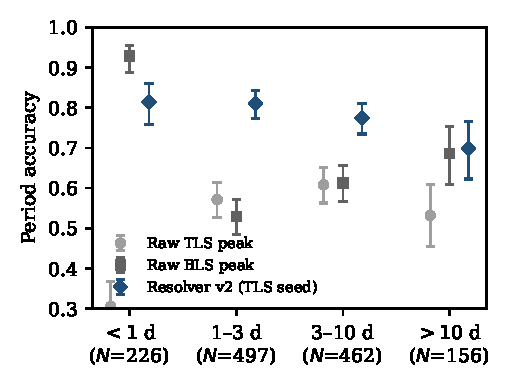
\includegraphics[width=\columnwidth]{figures/fig_b5_period.pdf}
\caption{B5: fraction of binaries in the main sample whose catalog period is recovered, by catalog period, for the raw TLS and BLS periods and for the resolver started from TLS, with 95\% Wilson intervals. The number under each bin is the number of binaries. The low TLS values at short periods are caused by the lower limit of its period grid (Section~\ref{sec:b5}).}
\label{fig:b5}
\end{figure}

\begin{deluxetable*}{lcccc}
\tablecaption{B5: alias resolution on TESS eclipsing binaries (primary sample). \label{tab:b5}}
\tablewidth{0pt}
\tablehead{\colhead{Method} & \colhead{Accuracy [95\% CI]} & \colhead{ECE} & \colhead{Abstain} & \colhead{McNemar vs.\ raw seed}}
\startdata
Raw TLS peak & 0.535 [0.508, 0.561] & \nodata & \nodata & \nodata \\
Raw BLS peak & 0.644 [0.618, 0.669] & \nodata & \nodata & \nodata \\
Resolver v2, TLS seed (primary) & 0.786 [0.763, 0.807] & 0.097 & 21.3\% & $418/81$, $p=1\times10^{-55}$ \\
Resolver v2, BLS seed & 0.792 [0.769, 0.813] & 0.084 & 22.1\% & $281/82$, $p=1\times10^{-26}$ \\
Resolver v1, TLS seed & 0.786 [0.763, 0.807] & 0.131 & 4.5\% & \nodata \\
\emph{First run (default stellar parameters, no F4)} &  &  &  &  \\
Raw TLS peak & 0.675 [0.649, 0.699] & \nodata & \nodata & \nodata \\
Resolver v2, TLS seed & 0.814 [0.793, 0.834] & 0.091 & 28.6\% & $254/67$, $p=9\times10^{-27}$ \\
\emph{Above the TLS period floor (754 binaries)} &  &  &  &  \\
Raw TLS peak & 0.682 [0.648, 0.714] & \nodata & \nodata & \nodata \\
Resolver v2, TLS seed & 0.779 [0.748, 0.807] & \nodata & \nodata & $137/64$, $p=3\times10^{-7}$
\enddata
\tablecomments{Primary sample: 1{,}341 eclipsing binaries with at least two early-window primary eclipses, excluding near-equal eclipses (B-amb). Accuracy is top-1 (no abstention); a period is correct if within 0.1\% of the catalog period. McNemar columns give discordant pairs won by the resolver / by the raw seed and the exact two-sided $p$. Against raw BLS the TLS-seeded resolver gives $281/90$, $p=5\times10^{-24}$.}
\end{deluxetable*}


\emph{A protocol error in the first run.} While checking our own results we found that the first B5 run did not follow the protocol. Our table of stellar parameters lacked TIC values for almost all B5 stars, so TLS used its default solar values and F4 was inactive. We reran TLS and the resolver with TIC values, as the protocol requires, and wrote down before the rerun that it would be the main result whatever it showed (Appendix~\ref{app:amend}). All numbers above are from the rerun. The first run gives the same conclusion: the resolver reaches \bFiveOrigAcc\ \bFiveOrigAccCI, against \bFiveOrigTls\ for TLS ($\bFiveOrigTlsFix/\bFiveOrigTlsBreak$, $p\bFiveOrigTlsP$) and \bFiveRawBls\ for BLS ($\bFiveOrigBlsFix/\bFiveOrigBlsBreak$, $p\bFiveOrigBlsP$).

\emph{Post hoc: why TLS does worse with real stellar radii.} TLS builds its period grid for a single star \citep{Ofir2014}. Its shortest trial period is that of an orbit three stellar radii wide, and the TIC radius of a binary is often large. For \bFiveFloorBelow\ of the \bFiveFloorKnown\ binaries with a TIC radius and mass, the catalog period is below this limit. TLS then cannot return it (\bFiveFloorBelowTls, against \bFiveFloorBelowOrig\ with default values) and usually returns a multiple. Of the \bFiveFloorLost\ binaries that TLS gets right only with default values, \bFiveFloorLostMult\ are at a whole multiple and \bFiveFloorLostGrid\ are within 1\% of the catalog period but outside 0.1\%, because the grid is coarser for stars of low density. TLS also crashed on \bFiveFloorTlsErr\ stars of the main sample, which count as wrong for TLS and for the resolver started from it. Part of the margin over TLS therefore comes from a search setting that does not suit binaries. The fair comparison uses the \bFiveFloorAboveN\ binaries whose period lies inside the grid, where the stellar parameters do not change the TLS result (\bFiveFloorAboveTls\ with TIC values, \bFiveFloorAboveOrig\ without). There the resolver reaches \bFiveFloorAboveAcc\ \bFiveFloorAboveAccCI, against \bFiveFloorAboveTls\ \bFiveFloorAboveTlsCI\ for TLS ($\bFiveFloorAboveTlsFix/\bFiveFloorAboveTlsBreak$, $p\bFiveFloorAboveTlsP$) and \bFiveFloorAboveBls\ for BLS ($p\bFiveFloorAboveBlsP$). Below the limit the resolver recovers \bFiveFloorBelowAcc, because its factors include $1/2$ and smaller. This subset analysis is post hoc in B5 and was repeated as a preregistered test in B6 (Section~\ref{sec:b6}).

\emph{Post hoc: the density test on binaries.} F4 assumes a transit across a single star of the TIC density, which is the wrong model for a binary. With the same BLS seeds, turning F4 on (it is active for \bFiveFourActive\ binaries) lowers the accuracy from \bFiveFourWithout\ to \bFiveFourWith\ ($\bFiveFourFix/\bFiveFourBreak$ in favor of leaving it out, $p\bFiveFourP$).

\emph{Post hoc: the rule based correction.} The correction of \citet{Tschudi2026a}, applied to the same TLS results, changes the TLS period for \bFiveTschChanged\ binaries of the main sample. It corrects \bFiveTschToRight\ and breaks \bFiveTschToWrong, so its accuracy (\bFiveTschAcc) equals that of raw TLS ($p\bFiveTschVsTlsP$). The resolver beats it with $\bFiveTschFix/\bFiveTschBreak$ ($p\bFiveTschP$). Its rules were tuned for planets around M dwarfs, not for binaries, so this shows only that the resolver's gain is not something an existing rule set already does.

\emph{Post hoc: SPOC periods.} SPOC found TCEs on \bFiveSpocStars\ of the \bFiveIncluded\ binaries. On each star we took the TCE whose period is within 1\% of an alias of the catalog period, the strongest one if there were several. This choice uses the truth and so favors SPOC. The single sector search of the first early sector then gives the catalog period for \bFiveSpocOne\ of the binaries in the main sample (it gives some period for \bFiveSpocOneCov\%), and the longest early search gives it for \bFiveSpocE\ (some period for \bFiveSpocECov\%). On the binaries where SPOC gives a period, it is correct for \bFiveSpocOneGiven\ and \bFiveSpocEGiven, and the resolver beats it with $\bFiveSpocOneGivenFix/\bFiveSpocOneGivenBreak$ ($p\bFiveSpocOneGivenP$) and $\bFiveSpocEGivenFix/\bFiveSpocEGivenBreak$ ($p\bFiveSpocEGivenP$). SPOC is built to find transit like signals and to flag binaries with tests such as odd and even depths, not to report the orbital period of a binary, so this does not measure SPOC at its own task.

\emph{Post hoc: periods from other sources.} \citet{Kostov2025} give TESS periods for \bFiveKostovN\ binaries of the main sample, which agree with the \citet{Prsa2022} period for \bFiveKostovCat. Scored against them, the resolver is correct for \bFiveKostovRes, TLS for \bFiveKostovTls\ and BLS for \bFiveKostovBls; the sample is too small to show a difference ($p\bFiveKostovP$). Gaia DR3 gives periods from its own photometry \citep{GaiaDR3,Mowlavi2023} for \bFiveGaiaN\ binaries of the main sample, and they agree with the catalog for \bFiveGaiaCat. Scored against Gaia, the resolver is correct for \bFiveGaiaRes, TLS for \bFiveGaiaTls\ ($p\bFiveGaiaTlsP$) and BLS for \bFiveGaiaBls\ ($p\bFiveGaiaBlsP$).

\subsubsection{Checking the catalog with later data} \label{sec:audit}

B5 scores against the catalog period, which is itself measured from data and can be wrong. Before any B5 light curve was downloaded, we planned an audit of every scored binary where the resolver's period differs from the catalog by more than 0.1\% (\auditN\ binaries, \auditBN\ in the main sample and \auditAmbN\ in B-amb). For each, the later sectors, which neither method had seen, are fitted at both periods with the same binary model: a primary and a secondary trapezoid, the secondary at a free phase, with the period refined locally and the same number of free parameters at both periods. A verdict needs $|\Delta\chi^2|>10$. Table~\ref{tab:audit} lists the results by the ratio of the two periods.

Later data favor the resolver's period for \auditVtwo\ binaries (\auditVtwoPc\%) and the catalog period for \auditCat\ (\auditCatPc\%). \auditInc\ (\auditIncPc\%) are undecided and \auditIns\ have too few later eclipses. Where the resolver chose half the catalog period (\auditHalfN\ cases), the later data rarely decide (\auditHalfInc\ undecided), as expected for nearly equal eclipses. Where it chose twice the catalog period (\auditDoubleN), later data favor the resolver in \auditDoubleVtwo\ cases and the catalog in \auditDoubleCat. In \auditNonaliasN\ cases the two periods are not related by a simple factor; \auditNonaliasClose\ of these differ by less than 1\%, and later data favor the resolver in \auditNonaliasVtwo\ and the catalog in \auditNonaliasCat. So the audit does not show that the catalog is usually wrong where the resolver disagrees with it: later data side with each about equally often. The B5 result is scored against the catalog as planned and is not changed by the audit.

In the first run the audit covered \auditFirstN\ disagreements. The audit code, model and thresholds did not change. Where the resolver's period is the same in both runs (\auditSamePeriod\ stars), the verdict is the same for \auditSameVerdict. The counts differ because the rerun produced a different set of disagreements; of the \auditOnlyNewN\ new ones, later data favor the catalog in \auditOnlyNewCat.

Of the binaries with a verdict, \auditDecidedToi\ host TOIs, most of them already marked as false positives, and \auditDecidedNea\ appears in the NASA Exoplanet Archive. The released table lists them all. Two need comment. TIC~92352621 is WASP-94~B, host of the planet WASP-94~B~b. The resolver's period for its catalog signal, \flagWaspRes\,d, matches the archive period of WASP-94~A~b (\flagWaspArchive\,d) on the neighboring star TIC~92352620. This signal is therefore probably the transit of that planet, diluted in the shared aperture and listed at twice its period, and not an eclipsing binary; matching ephemerides is the standard way to find such contamination \citep{Coughlin2014}. TIC~354518617 hosts the confirmed planet TOI-2540.01, whose period (\flagToiPeriod\,d) has nothing to do with the \flagToiCat\,d and \flagToiRes\,d periods compared here.

We release the cases with a verdict as candidate period revisions (Appendix~\ref{app:data}). They are not confirmed revisions, and each should be checked against the light curve and the binary's other data before an ephemeris is changed.

Figure~\ref{fig:lc} shows one case with a verdict, TIC~\lcTic. The catalog period is \lcPcat\,d. The TLS search of the early data found \lcPseed\,d, and the resolver kept that period with probability \lcProb. Folded at the catalog period, the odd and even eclipses of the early data have clearly different depths (panel a). Compared with the chosen period, the catalog period scores better on events where they are predicted (F1, \lcDFOne) but worse on odd and even depths (F2, \lcDFTwo) and on the secondary eclipse (F3, \lcDFThree), because at twice the catalog period the shallower events become a secondary eclipse at phase 0.5 (panel b). The later sectors, which the resolver did not see, show a primary and a shallower secondary eclipse at the resolver's period (panel c), and the audit prefers that period by $\Delta\chi^2 = \lcDchi$.

\begin{figure*}[t]
\centering
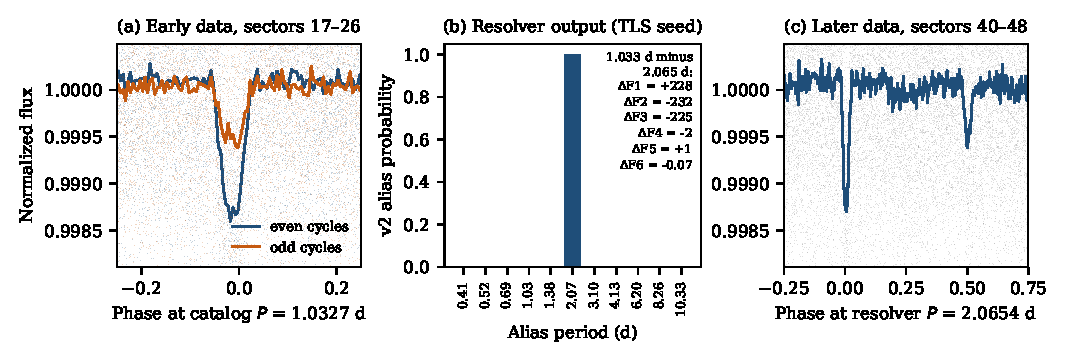
\includegraphics[width=\textwidth]{figures/fig_lc_example.pdf}
\caption{An audit case, TIC~\lcTic. (a) Early light curve (\lcEarlyN\ sectors, \lcEarlySec), the data given to the searches and to the resolver, folded at the catalog period of \lcPcat\,d; lines are binned medians of even and odd cycles. (b) Probabilities of the frozen \Vtwo\ resolver started from the TLS period, and the six tests of the catalog period minus those of the chosen period (natural log likelihood). (c) The first \lcLaterN\ later sectors (\lcLaterSec), not seen by the resolver, folded at the resolver's period of \lcPres\,d. The audit used all later sectors.}
\label{fig:lc}
\end{figure*}

\begin{deluxetable*}{lrrrrr}
\tablecaption{Catalog-truth audit of B5 disagreements (secondary analysis). \label{tab:audit}}
\tablewidth{0pt}
\tablehead{\colhead{Relation} & \colhead{$N$} & \colhead{Favors resolver} & \colhead{Favors catalog} & \colhead{Inconclusive} & \colhead{Insufficient}}
\startdata
$P_{\rm res}=P_{\rm cat}/2$ & 152 & 9 & 24 & 117 & 2 \\
$P_{\rm res}=2P_{\rm cat}$ & 108 & 29 & 27 & 47 & 5 \\
$P_{\rm res}=4P_{\rm cat}$ & 3 & 0 & 2 & 0 & 1 \\
not an alias & 97 & 40 & 26 & 23 & 8 \\
All & 360 & 78 & 79 & 187 & 16
\enddata
\tablecomments{Each disagreement between the resolver and the catalog period was tested on the later-sector light curve by fitting the same eclipsing-binary model (primary and free-phase secondary) at both periods; a decision requires $|\Delta\chi^2|>10$. The decided cases are released as candidate period revisions, not confirmations.}
\end{deluxetable*}


\subsection{B6: a preregistered replication} \label{sec:b6}

Three things left the B5 result less certain than we wanted: the run had to be repeated, the comparison with TLS inside its period grid was post hoc, and the comparison of the resolver started from BLS with raw BLS was only secondary. Before downloading any more data, we therefore wrote down a replication on the \bSixIncluded\ binaries that B5 left out at random. Selection, data, searches, resolver and scoring are exactly those of the B5 rerun. Three hypotheses were fixed in advance, each to be tested with an exact McNemar test at $p<0.01/3$ to allow for testing three: the B5 goal (H1), the resolver against TLS on binaries inside the TLS period grid (H2), and the resolver started from BLS against raw BLS (H3). The scoring code was committed before the searches finished, and it was run once.

All three hypotheses hold (Table~\ref{tab:b6}). On the \bSixN\ binaries of the main sample the resolver returns the catalog period for \bSixAcc\ \bSixAccCI, against \bSixTls\ for TLS ($\bSixHoneTlsFix/\bSixHoneTlsBreak$, $p\bSixHoneTlsP$) and \bSixBls\ for BLS ($\bSixHoneBlsFix/\bSixHoneBlsBreak$, $p\bSixHoneBlsP$). Inside the TLS grid (\bSixHtwoN\ binaries) it reaches \bSixHtwoAcc\ against \bSixHtwoTls\ ($\bSixHtwoFix/\bSixHtwoBreak$, $p\bSixHtwoP$). Started from BLS it reaches \bSixAccBlsSeed\ against \bSixBls\ ($p\bSixHthreeP$). TLS crashed on \bSixTlsErr\ stars, which count as wrong.

The predictions written down with the protocol also hold. The probabilities are again too confident on binaries (ECE \bSixEce). The simple sum of the six tests (\bSixSum) is as accurate as the learned combiner (\bSixLearned). Leaving out the density test does not lower the accuracy (\bSixNoFfour), while leaving out F1 or F2 does (\bSixNoFone\ and \bSixNoFtwo). The audit with later data, repeated unchanged on the \bSixAuditN\ B6 binaries where the resolver disagrees with the catalog, again splits about evenly: later data favor the resolver in \bSixAuditRes, the catalog in \bSixAuditCat, and \bSixAuditInc\ are undecided. Taken together, the \poolN\ binaries of the B5 and B6 main samples give \poolAcc\ \poolAccCI\ for the resolver, \poolTls\ for TLS and \poolBls\ for BLS, and \poolGridAcc\ against \poolGridTls\ inside the TLS grid (\poolGridN\ binaries).

\begin{deluxetable*}{lrllcccc}
\tablecaption{B6: preregistered replication on binaries not used in B5. \label{tab:b6}}
\tablewidth{0pt}
\tablehead{\colhead{} & \colhead{$N$} & \colhead{Seed} & \colhead{Against} & \colhead{Resolver} & \colhead{Baseline} & \colhead{McNemar} & \colhead{Pass}}
\startdata
H1 & 1{,}597 & TLS & raw TLS & 0.780 [0.759, 0.800] & 0.545 [0.520, 0.569] & $487/111$, $p=4\times10^{-57}$ & yes \\
H1 & 1{,}597 & TLS & raw BLS & 0.780 [0.759, 0.800] & 0.626 [0.602, 0.650] & $370/124$, $p=2\times10^{-29}$ & yes \\
H2 & 935 & TLS & raw TLS$^a$ & 0.773 [0.745, 0.799] & 0.662 [0.631, 0.692] & $201/97$, $p=2\times10^{-9}$ & yes \\
H3 & 1{,}597 & BLS & raw BLS & 0.785 [0.764, 0.805] & 0.626 [0.602, 0.650] & $364/110$, $p=9\times10^{-33}$ & yes
\enddata
\tablecomments{Accuracy with 95\% Wilson intervals. Each hypothesis passes if the resolver wins the exact paired McNemar test with $p<0.0033$ (0.01 divided by three hypotheses). Discordant pairs are given as won by the resolver / won by the baseline. $^a$Binaries whose catalog period lies inside the TLS period grid. All four tests were specified before any B6 light curve was downloaded.}
\end{deluxetable*}


\subsection{B1: injected signals} \label{sec:b1}

Table~\ref{tab:b1} gives the B1 test results. Started from wrong periods, of which only \bOneWSeed\ are already correct (the case $r=1$), the resolver recovers the true period for \bOneWAcc\ \bOneWAccCI\ of \bOneWN\ injections. Its \Vone\ ECE is \bOneWEceVone, which meets the preregistered goal of an ECE below 0.05, and its accuracy on the 90\% of injections it is most confident about is \bOneWAccNinety. Accuracy ranges from \bOneAliasMin\ to \bOneAliasMax\ across the eleven factors (Figure~\ref{fig:b1}). Binaries with equal eclipses are the hardest case (\bOneTwinAcc, against \bOnePlanetAcc\ for planets). The simple combiner, which cannot separate such binaries (Section~\ref{sec:combine}), reaches \bOneTwinPr\ on them and \bOneWPr\ overall, and the learned combiner is better on the same injections ($p\bOneLearnVsPrP$). Accuracy also depends on how many events the data cover: \bOneEpochFew\ with at most one event and \bOneEpochMany\ with four or more.

Started from real search periods, the picture is less good. The BLS and TLS periods are correct for \bOneBSeed\ and \bOneTSeed\ of the 2{,}000 searched injections. The resolver raises this to \bOneBAcc\ \bOneBAccCI\ and \bOneTAcc\ \bOneTAccCI\ ($\bOneBMcFix/\bOneBMcBreak$ and $\bOneTMcFix/\bOneTMcBreak$, $p\bOneBMcP$ and $p\bOneTMcP$). The ceiling is \bOneBCeil\ and \bOneTCeil: in the other cases the search found a period unrelated to the true one, and no choice among the factors can help. For \bOneFloorBelow\ of the \bOneFloorN\ searched injections the injected period is below the TLS grid limit, so TLS could not find it; the same holds for \bTwoFloorBelow\ of the \bTwoFloorN\ B2 TOIs with TIC values. With search seeds the \Vone\ ECE is \bOneBEceVone\ (BLS) and \bOneTEceVone\ (TLS), so \Vone\ misses the calibration goal there. The post hoc \Vtwo\ calibration gives \bOneBEceVtwo\ and \bOneTEceVtwo, gives no answer for \bOneBAbstVtwo\% and \bOneTAbstVtwo\% of these injections, and is \bOneBNaVtwo\ and \bOneTNaVtwo\ correct where it answers. On wrong period seeds, which it was not fitted on, \Vtwo\ has an ECE of \bOneWEceVtwo. Figure~\ref{fig:rel} shows these calibrations and those of B2 and B5.

\begin{figure*}[t]
\centering
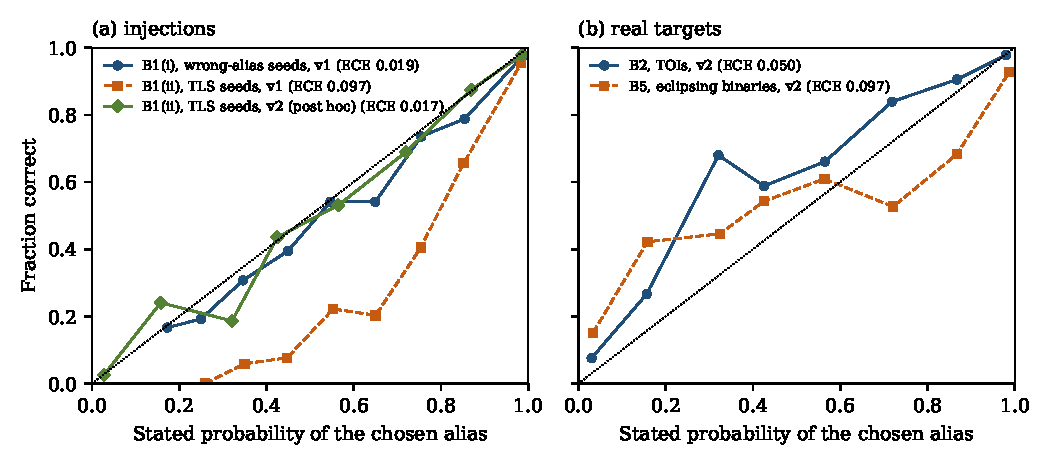
\includegraphics[width=0.9\textwidth]{figures/fig_reliability.pdf}
\caption{Reliability diagrams: the fraction of targets whose chosen period is correct, against the probability the resolver gives for it, in the ten bins used for the ECE (bins with fewer than 20 targets are not drawn). (a) B1 test injections, started from wrong periods with \Vone, and from TLS periods with \Vone\ and with the post hoc \Vtwo. (b) Real targets with \Vtwo: the B2 TOIs and the B5 binaries. The dotted line is perfect calibration. The ECE values are those of Tables~\ref{tab:b1}, \ref{tab:b2} and \ref{tab:b5}.}
\label{fig:rel}
\end{figure*}

\begin{figure}[t]
\centering
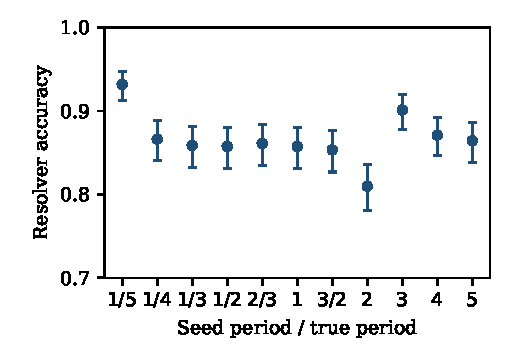
\includegraphics[width=\columnwidth]{figures/fig_b1_alias.pdf}
\caption{B1(i): resolver accuracy on the \bOneWN\ test injections for each factor between the seed period and the true period, with 95\% Wilson intervals. At $r=1$ the seed is already correct.}
\label{fig:b1}
\end{figure}

\begin{deluxetable*}{lrccccc}
\tablecaption{B1: injection-recovery test split. \label{tab:b1}}
\tablewidth{0pt}
\tablehead{\colhead{Seed} & \colhead{$N$} & \colhead{Seed alone} & \colhead{Resolver accuracy [95\% CI]} & \colhead{ECE v1} & \colhead{ECE v2$^a$} & \colhead{Ceiling}}
\startdata
Wrong alias seed & 8{,}620 & 0.091 & 0.866 [0.859, 0.873] & 0.019 & 0.056 & 0.971 \\
BLS search seed & 2{,}000 & 0.644 & 0.784 [0.765, 0.801] & 0.096 & 0.014 & 0.831 \\
TLS search seed & 2{,}000 & 0.608 & 0.791 [0.773, 0.809] & 0.097 & 0.017 & 0.849
\enddata
\tablecomments{Accuracy and v1 ECE are pre-registered results scored after the v1 freeze. $^a$v2 ECE is post hoc: v2 was defined after the v1 search-seed results were known. Accuracy is identical for v1 and v2 by construction. Ceiling: fraction of injections for which one of the eleven refined candidates matches the truth.}
\end{deluxetable*}


\subsection{B2: TOIs held out in time} \label{sec:b2}

B2 asks whether the gains on simulated signals and binaries carry over to the TOI catalog. The goal was that the resolver started from TLS (\Vtwo) beats raw BLS, raw TLS and SPOC-1, each with McNemar $p<0.01$. It is not met (Table~\ref{tab:b2}). The resolver is correct for \bTwoAcc\ \bTwoAccCI\ of \bTwoN\ TOIs, against \bTwoRawTls\ for TLS ($\bTwoMcTlsFix/\bTwoMcTlsBreak$, $p\bTwoMcTlsP$) and \bTwoRawBls\ for BLS ($\bTwoMcBlsFix/\bTwoMcBlsBreak$, $p\bTwoMcBlsP$). On TOIs it is comparable to the two searches and does not improve on them. The rule based correction of \citet{Tschudi2026a} matches TLS (\bTwoRawTsch), because its rules rarely trigger here: it changes the TLS period for \bTwoTschDiffer\ of the \bTwoTschCompared\ TOIs searched. SPOC-1 and SPOC-E give a period for \bTwoCovSpocOne\% and \bTwoCovSpocE\% of TOIs, and the resolver's lead over them in Table~\ref{tab:b2} comes only from that. Where SPOC gives a period it is at least as accurate as the resolver: \bTwoGivenSpocOne\ for SPOC-1 ($\bTwoMcGivenSpocOneFix/\bTwoMcGivenSpocOneBreak$, $p\bTwoMcGivenSpocOneP$) and \bTwoGivenSpocE\ for SPOC-E ($\bTwoMcGivenSpocEFix/\bTwoMcGivenSpocEBreak$, $p\bTwoMcGivenSpocEP$). The same holds for the published QLP and SPOC catalog periods.

When the resolver starts from a period that is usually right already, it turns more correct periods into wrong ones than the other way round. Started from BLS it corrects \bTwoSelfBlsFix\ and breaks \bTwoSelfBlsBreak\ BLS periods ($p\bTwoSelfBlsP$), and started from SPOC-E it corrects \bTwoSelfSpocEFix\ and breaks \bTwoSelfSpocEBreak\ ($p\bTwoSelfSpocEP$). The resolver and TLS are correct for \bTwoTierAAcc\ and \bTwoTierATls\ of planets ($p\bTwoTierAP$) and for \bTwoTierBAcc\ and \bTwoTierBTls\ of binaries ($p\bTwoTierBP$). The ECE is \bTwoEce\ overall and \bTwoTierBEce\ for the binaries.

\emph{Exploratory: TOIs with one sector.} Among TOIs with a single early sector, which was not in the protocol, the resolver is correct for \bTwoOneSecAcc\ against \bTwoOneSecTls\ for TLS ($p\bTwoOneSecP$, \bTwoOneSecN\ TOIs). This is one of \bTwoStrataN\ groups by number of sectors. With a correction for testing that many groups the difference remains ($p\bTwoOneSecPBonf$), but in the groups with 2 to 3, 4 to 6 and 7 to 12 sectors the resolver is slightly below TLS (\bTwoStrTwoThreeAcc\ against \bTwoStrTwoThreeTls, \bTwoStrFourSixAcc\ against \bTwoStrFourSixTls, and \bTwoStrSevenTwelveAcc\ against \bTwoStrSevenTwelveTls), and none of those differences is significant. The result for single sectors should be treated as a hypothesis for a future preregistered test.

\begin{deluxetable*}{lcccc}
\tablecaption{B2: temporal holdout on TOIs (primary sample). \label{tab:b2}}
\tablewidth{0pt}
\tablehead{\colhead{Method} & \colhead{Coverage} & \colhead{Accuracy [95\% CI]} & \colhead{Resolver vs.\ method} & \colhead{Same, where method gives a period}}
\startdata
Resolver v2, TLS seed & 100.0\% & 0.832 [0.810, 0.853] & \nodata & \nodata \\
Raw TLS peak & 99.8\% & 0.814 [0.791, 0.836] & $69/48$, $p=0.064$ & $69/48$, $p=0.064$ \\
Raw BLS peak & 100.0\% & 0.826 [0.804, 0.847] & $60/53$, $p=0.573$ & $60/53$, $p=0.573$ \\
Tschudi (2026a) correction & 99.8\% & 0.814 [0.791, 0.836] & $68/47$, $p=0.062$ & $68/47$, $p=0.062$ \\
SPOC TCE, single sector & 72.6\% & 0.675 [0.648, 0.701] & $239/55$, $p=2\times10^{-28}$ & $37/55$, $p=0.076$ \\
SPOC TCE, multiple sector & 82.4\% & 0.765 [0.740, 0.788] & $148/69$, $p=9\times10^{-8}$ & $41/69$, $p=0.010$ \\
QLP (G21 catalog) & 5.1\% & 0.050 [0.039, 0.064] & $925/10$, $p=9\times10^{-259}$ & $1/10$, $p=0.012$ \\
SPOC (G21 catalog) & 45.9\% & 0.439 [0.411, 0.467] & $517/57$, $p=9\times10^{-94}$ & $10/57$, $p=4\times10^{-9}$
\enddata
\tablecomments{1{,}169 TOIs with Tier A or B truth and at least two transits in the early window. A method that gives no period counts as wrong; the last column restricts to TOIs where it gives one. McNemar entries: discordant pairs won by the resolver / by the method, exact two sided $p$.}
\end{deluxetable*}


\emph{Post hoc: answering only when confident.} The resolver gives no answer for \bTwoAbst\% of B2 TOIs. On the \selAnswered\ it answers it is \selOurs\ correct, against \selTls\ for TLS ($p\selTlsP$) and \selBls\ for BLS ($p\selBlsP$) on the same TOIs. On the \abstN\ TOIs without an answer all methods do poorly (resolver \abstOurs, TLS \abstTls, BLS \abstBls), so abstaining picks out hard targets. Most of this, however, is already in the TLS detection strength. Keeping the same fraction of TOIs ranked by TLS SDE gives \rcTls, close to the resolver's \rcOurs, and the area under the accuracy against coverage curve is \aucOurs\ for the resolver and \aucTls\ for TLS ranked by SDE (Figure~\ref{fig:riskcov}). What the resolver adds is a probability for each period and a calibrated choice to abstain.

\begin{figure}[t]
\centering
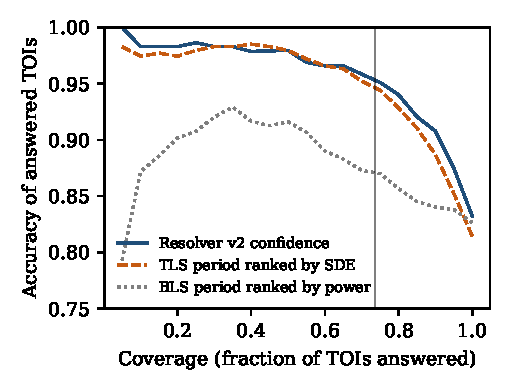
\includegraphics[width=\columnwidth]{figures/fig_b2_riskcov.pdf}
\caption{B2 (post hoc): accuracy of the answered TOIs against the fraction answered, when TOIs are ranked by the \Vtwo\ probability, by the TLS SDE of the raw TLS period, or by the BLS power of the raw BLS period. The vertical line marks the coverage at the \Vtwo\ threshold.}
\label{fig:riskcov}
\end{figure}

\emph{Post hoc: why B2 differs from B1 and B5.} In B2 the raw TLS period is already correct for \cmpTlsBTwo\ of targets, against \cmpTlsBOne\ for the B1(ii) injections. Only \cmpEbBTwo\% of B2 targets are binaries, against \cmpEbBOne\% of the B1(ii) injections, and TOIs were chosen because a search had already found them at a usable period. There is little room for alias correction, and most of the remaining errors are not aliases (the ceiling for TLS seeds is \bTwoCeilTls).

\emph{Post hoc: the dropped TOI audit (B3).} We had planned an audit (B3) that would flag TOIs where the resolver confidently disagrees with the current catalog period. Among the \nogoN\ B2 TOIs where that happens, the resolver is right for a fraction \nogoRight\ and the catalog for \nogoCatRight, so such an audit would mostly flag correct periods. We dropped it.

\emph{Post hoc: how often TOI periods were changed by an alias factor.} The TOI catalog of the first two years \citep{Guerrero2021} lists \revHist\ TOIs, and \revBoth\ have a period both there and in the ExoFOP table of 2026 September 30. For \revAlias\ of them (\revAliasPc\% \revAliasCI) the current period is within 1\% of an alias of the published one (\revDouble\ doubled, \revHalf\ halved), and \revOther\ changed by some other amount. Of the \revAlias, \revAliasFp\ are now marked as false positives or false alarms, \revAliasCp\ are confirmed or known planets and \revAliasOpen\ are still candidates; \revAliasEb\ are in an EB catalog. The share of false positives among them (\revAliasFpPc\%) is close to that among TOIs whose period did not change (\revSameFpPc\%). Alias changes of released TOIs are therefore uncommon and are not concentrated in false positives.

\emph{Post hoc: TOIs at half the period of a known binary.} Of \bTwoHalfTotal\ TOIs with a period, \bTwoHalfSame\ match the period of a cataloged binary on the same star \citep{Prsa2022,Kostov2025} within 1\%, and \bTwoHalfN\ sit at half of it. Of those \bTwoHalfN, \bTwoHalfFp\ are already marked as false positives or false alarms, \bTwoHalfCp\ are confirmed or known planets, for which the match may say nothing about the planet, and \bTwoHalfOpen\ are still open. Correcting open TOIs at half a binary period therefore concerns about that many targets.

\emph{Post hoc: planets with a secondary event.} To check that F3 does not move planets with an occultation to a wrong period, we took the B2 planets in which the resolver finds a secondary event with S/N of at least 5 (\occN\ TOIs). For \occNoCand\ of them the true period is not among the candidates, so the ``secondary'' is a side effect of folding at an unrelated period. For the \occTrueN\ where it is seen at the true period, the resolver is correct for \occTrueRes\ and TLS for \occTrueTls. Over all \occN, the resolver and TLS differ on two TOIs ($\occFix/\occBreak$). The sample is small, but it shows no sign that a secondary event moves a planet to a wrong period.

\subsection{False alarms} \label{sec:fa}

To see how the resolver behaves when there is no real signal, we ran it on the early light curves of the \faScrN\ B2 candidates (before the transit count check) after either inverting the flux ($f \to 2-f$, which turns dips into bumps) or scrambling it (shuffling blocks of one day within each stretch of continuous data). The seed is the BLS period of the changed light curve. The goal was that the resolver be confident on fewer than 5\% of scrambled light curves. It is missed (Table~\ref{tab:fa}). \Vtwo\ is confident for \faScrVtwo\% \faScrVtwoCI\ of scrambled and \faInvVtwo\% \faInvVtwoCI\ of inverted light curves; \Vone\ and the simple combiner are confident more often. The seeds of scrambled light curves have a median period of \faScrSeedMed\,d, against \faInvSeedMed\,d for inverted ones. Scrambling keeps the variability within each day, and shuffled blocks of it can line up into dips that repeat at a regular spacing. The resolver assumes the signal is real and has no test of that, so it treats such dips like eclipses.

\emph{Post hoc: the searches on the same light curves.} To see whether the resolver adds false confidence beyond the search itself, we recorded how often the searches reach SDE\,$\ge$\,9 on the same light curves (Table~\ref{tab:fa}). TLS does so for \ctxScrTls\% \ctxScrTlsCI\ of scrambled and \ctxInvTls\% \ctxInvTlsCI\ of inverted light curves. The BLS search that supplied each seed, with SDE computed as for the injection hosts, does so for \ctxScrAsix\% \ctxScrAsixCI\ and \ctxInvAsix\% \ctxInvAsixCI. Both searches pass on the same light curve for \ctxScrSdeAnd\% of scrambled and \ctxInvSdeAnd\% of inverted light curves, and at least one passes for \ctxScrSdeOr\% and \ctxInvSdeOr\%. Over the whole sample, the resolver is therefore confident less often than either search passes a standard detection threshold. It does not pick the same light curves, however. Among scrambled light curves with TLS SDE\,$\ge$\,9 it is confident for \ctxScrTlsBoth\%, and among those below that threshold still for \ctxScrTlsLow\% (\ctxScrTlsLowN\ light curves); for inverted light curves the rates are \ctxInvTlsBoth\% and \ctxInvTlsLow\%. Requiring both TLS SDE\,$\ge$\,9 and a confident answer leaves \ctxScrTlsJoint\% of scrambled and \ctxInvTlsJoint\% of inverted light curves. On scrambled data the resolver gives confident answers on signals the search would not have passed, so it adds false confidence there, and neither statistic alone rejects such signals.

Tools built for this task do far better. LEO-Vetter rejects \litLeoReject\% of simulated false alarms from scrambled light curves while passing \litLeoPass\% of injected planets \citep[][their Section~\litLeoSec]{Kunimoto2025leo}, and ExoMiner++ reaches a precision of \litExoPrec\ at a recall of \litExoRec\ on labeled TESS 2 minute TCEs \citep[][their Table~\litExoTab]{Valizadegan2025}. The resolver is not a false alarm filter and does not compete with such tools. It belongs after them; its own question, which period a vetted signal has, is the one tested in the benchmarks above.

\begin{deluxetable*}{lrccccc}
\tablecaption{False-alarm test: fraction of light curves resolved with confidence. \label{tab:fa}}
\tablewidth{0pt}
\tablehead{\colhead{Light curves} & \colhead{$N$} & \colhead{v2 [95\% CI]} & \colhead{v1} & \colhead{Principled} & \colhead{TLS SDE$\ge9^a$} & \colhead{BLS SDE$\ge9^a$}}
\startdata
Scrambled & 1{,}198 & 37.2\% [34.5, 40.0] & 67.0\% & 43.7\% & pending & pending \\
Inverted & 1{,}198 & 4.0\% [3.0, 5.3] & 18.6\% & 7.5\% & pending & pending
\enddata
\tablecomments{The pre-registered criterion is a confident-resolution rate below 5\% on scrambled light curves. $^a$Post hoc: the rate at which the searches themselves exceed SDE~$=9$ on the same light curves (BLS: TLS-style detrended SDE, amendment A6).}
\end{deluxetable*}


\subsection{B4: run time on a full sector} \label{sec:b4}

To measure speed we processed all \bFourPinned\ SPOC 2 minute light curves of Sector 49, of which \bFourN\ completed every step. Each light curve was read, cleaned and binned, searched with the GPU BLS, and passed with its BLS period to the frozen \Vtwo\ resolver (Table~\ref{tab:b4}). The search ran on NVIDIA \bFourGpu\ GPUs and the resolver on Kaggle sessions with \bFourCores\ virtual cores (\bFourCpuRes), as four separate processes. Per light curve the median total time is \bFourTotalMed\,s and the 95th percentile \bFourTotalPnf\,s, of which the resolver takes a median of \bFourResMed\,s. Summed over the parallel sessions, the search used \bFourBlsWallH\,h of GPU time and the resolver \bFourResWallH\,h of CPU time. Stellar densities for F4 were available for \bFourStellar\ of the stars. TLS was not run on this sample; on the B2 light curves it took a median of \bFourTlsMed\,s and a 95th percentile of \bFourTlsPnf\,s per light curve on four cores, so a TLS seeded run of a sector would be dominated by the search. These numbers describe a period check of one signal after detection. They cannot be compared with the cost of SPOC or QLP, which includes photometry, correction of instrumental effects, searches for several planets and vetting.

\begin{deluxetable*}{lccl}
\tablecaption{B4: processing time per light curve, TESS Sector 49. \label{tab:b4}}
\tablewidth{0pt}
\tablehead{\colhead{Stage} & \colhead{Median (s)} & \colhead{95th percentile (s)} & \colhead{Hardware}}
\startdata
Read light curve & 0.09 & 0.18 & GPU session host \\
Detrend and bin & 0.39 & 0.53 & GPU session host \\
BLS seed search & 1.01 & 1.09 & Tesla T4 \\
Alias resolver (v2) & 3.12 & 5.47 & CPU session \\
Total & 4.56 & 6.98 & \nodata
\enddata
\tablecomments{19{,}997 light curves. GPU session: one process per NVIDIA Tesla T4; CPU session: 4 vCPU (Intel(R) Xeon(R) CPU @ 2.20GHz), four worker processes with one BLAS thread each.}
\end{deluxetable*}


\subsection{Post hoc diagnostics} \label{sec:diag}

The analyses in this section were designed after the benchmark results were known. Their designs were written to the decision log before they were run. They use the frozen resolver without refitting and change no main result.

\emph{Match tolerance.} Table~\ref{tab:tol} repeats the main comparisons with tolerances of 0.05\%, 0.2\% and 0.5\% instead of 0.1\%. The B5 goal is met at every tolerance ($p\tolFiveMaxP$ or smaller for both comparisons), and the B1 accuracies change by less than two percentage points. In B2 the resolver, TLS and BLS remain comparable at 0.2\% and 0.5\% (\tolTwoLooseAcc, \tolTwoLooseTls\ and \tolTwoLooseBls\ at 0.2\%). At 0.05\% the resolver is ahead (\tolTwoTightAcc\ against \tolTwoTightTls\ for TLS and \tolTwoTightBls\ for BLS; $p\tolTwoTightTlsP$ and $p\tolTwoTightBlsP$). That reflects precision, not the choice of alias: the resolver refines each period, while a search returns the nearest point of its grid. It does not change the B2 result at the preregistered tolerance.

\begin{deluxetable*}{lcccc}
\tablecaption{Post hoc: accuracy as a function of the period match tolerance. \label{tab:tol}}
\tablewidth{0pt}
\tablehead{\colhead{Sample and method} & \colhead{0.05\%} & \colhead{0.1\% (primary)} & \colhead{0.2\%} & \colhead{0.5\%}}
\startdata
\emph{B1(i), wrong period seeds} &  &  &  &  \\
Resolver & 0.852 & 0.866 & 0.873 & 0.875 \\
\emph{B1(ii), TLS seeds} &  &  &  &  \\
Raw TLS peak & 0.562 & 0.608 & 0.614 & 0.618 \\
Resolver & 0.783 & 0.791 & 0.796 & 0.798 \\
\emph{B5, eclipsing binaries} &  &  &  &  \\
Raw TLS peak & 0.418 & 0.535 & 0.584 & 0.600 \\
Raw BLS peak & 0.610 & 0.644 & 0.665 & 0.683 \\
Resolver & 0.761 & 0.786 & 0.802 & 0.815 \\
\emph{B2, TOI holdout} &  &  &  &  \\
Raw TLS peak & 0.672 & 0.814 & 0.850 & 0.857 \\
Raw BLS peak & 0.760 & 0.826 & 0.840 & 0.847 \\
SPOC-1 & 0.650 & 0.675 & 0.683 & 0.688 \\
Resolver & 0.804 & 0.832 & 0.842 & 0.848
\enddata
\tablecomments{The 0.1\% column reproduces the preregistered results. The frozen resolver's chosen alias is the same in every column; only the test of correctness changes.}
\end{deluxetable*}


\emph{Which tests matter.} Table~\ref{tab:abl} gives the accuracy of the simple combiner when one of the six tests is left out. F1 carries most of the information in both samples. F2 and F3 come next and matter far more for binaries (\ablFiveFtwo\ and \ablFiveFthree\ without them, from \ablFiveAll) than for the injections, which are mostly planets. F5 and F6 change the accuracy by less than one percentage point. F4 adds little on injections and lowers the accuracy on binaries (\ablFiveFfour\ without it), as found above. The learned combiner relies mainly on the simple combiner's score, as permuting that score shows, and on injections it also uses the density information. On B5 the simple combiner (\ablFiveAll) is as accurate as the learned one (\ablFiveLearned\ on the same binaries); the learned combiner is better on injections (\ablOneLearned\ against \ablOneAll) and in calibration.

\begin{deluxetable*}{lcccc}
\tablecaption{Post hoc: contribution of each test. \label{tab:abl}}
\tablewidth{0pt}
\tablehead{\colhead{} & \colhead{Simple, B1(i)} & \colhead{Simple, B5} & \colhead{Learned, B1(i)} & \colhead{Learned, B5}}
\startdata
All six terms & 0.775 & 0.800 & \nodata & \nodata \\
without F1, predicted event coverage & 0.316 ($-$0.459) & 0.241 ($-$0.559) & $-$0.015 & $+$0.000 \\
without F2, odd/even depth & 0.691 ($-$0.085) & 0.475 ($-$0.324) & $-$0.004 & $-$0.007 \\
without F3, secondary eclipse & 0.748 ($-$0.028) & 0.667 ($-$0.133) & $-$0.023 & $-$0.004 \\
without F4, stellar density & 0.772 ($-$0.003) & 0.818 ($+$0.019) & $-$0.108 & $+$0.009 \\
without F5, ephemeris coherence & 0.785 ($+$0.009) & 0.800 ($+$0.001) & $-$0.012 & $-$0.007 \\
without F6, shape of alternating events & 0.776 ($+$0.001) & 0.800 ($+$0.000) & $-$0.007 & $+$0.002 \\
simple posterior permuted & \nodata & \nodata & $-$0.525 & $-$0.298
\enddata
\tablecomments{Columns 2 to 3: accuracy of the simple combiner with one test left out (change in parentheses), on the B1(i) test injections and the B5 primary sample. Columns 4 to 5: change in accuracy of the frozen learned combiner when the test and its inputs are permuted between targets (mean of five permutations). The learned combiner also sees the simple posterior, which contains all six terms, so its single test values are lower limits. Nothing was refitted.}
\end{deluxetable*}


\emph{Where the B5 errors come from.} Table~\ref{tab:err} assigns each of the \bFiveErrN\ binaries of the main sample with a wrong period to the first category that applies. For \bFiveErrNoCand\ (\bFiveErrNoCandPc\%) the true period was not among the candidates, so the search made the error and no choice of factor could repair it. The rest are wrong choices among the candidates: \bFiveErrTwin\ binaries with nearly equal eclipses, \bFiveErrEcc\ eccentric systems, \bFiveErrFew\ with at most three eclipses, \bFiveErrSnr\ with a seed S/N below 20, and \bFiveErrOther\ with none of these. Against an overall error rate of \bFiveErrRate\%, the rate is \bFiveErrRateTwin\% for nearly equal eclipses, \bFiveErrRateEcc\% for eccentric systems, \bFiveErrRateFew\% with at most three eclipses and \bFiveErrRateSnr\% at low S/N.

\begin{deluxetable*}{lrr}
\tablecaption{Post hoc: the 287 B5 primary binaries for which the resolver period is wrong. \label{tab:err}}
\tablewidth{0pt}
\tablehead{\colhead{Category (first that applies)} & \colhead{$N$} & \colhead{Share}}
\startdata
TLS search failed & 3 & 1.0\% \\
True period not a candidate, below the TLS period floor & 13 & 4.5\% \\
True period not a candidate, other & 106 & 36.9\% \\
Nearly equal eclipses (depth ratio $>0.8$) & 41 & 14.3\% \\
Eccentric (secondary $>0.05$ from phase 0.5) & 18 & 6.3\% \\
At most three eclipses in the early window & 10 & 3.5\% \\
Seed S/N below 20 & 60 & 20.9\% \\
None of the above & 36 & 12.5\%
\enddata
\tablecomments{Categories were fixed before counting and are applied in the order listed. Depth ratios and secondary phases are from the catalog of \citet{Prsa2022}.}
\end{deluxetable*}


%% ======================================================================
\section{Limitations} \label{sec:limits}

\emph{Real signals only.} The resolver chooses among periods of a signal it assumes is real. On scrambled light curves it is confident for \faScrVtwo\% of targets (Section~\ref{sec:fa}). It should be used only on signals that have passed vetting, and its confidence is not evidence that a signal is astrophysical.

\emph{Limited by the search.} The resolver only considers the eleven factors of the seed. When a search finds a peak unrelated to the true period, no choice of factor can recover it. This happened for \bOneTMissPc\% of the TLS seeds and \bOneBMissPc\% of the BLS seeds in B1(ii), for \bTwoMissTlsPc\% of the TLS seeds in B2 and for \bFiveMissTlsPc\% in B5, where it causes \bFiveErrNoCandPc\% of the resolver's errors. Periods related by other ratios, as in some systems with several planets, are outside this model.

\emph{Seeds that are usually right.} When the seed is already correct for most targets, as for BLS, SPOC and catalog periods in B2, the resolver turns more correct periods into wrong ones than the reverse (Section~\ref{sec:b2}). It should not be run over catalog periods in the hope of improving them. Its probabilities are more useful as a flag for review.

\emph{Probabilities on binaries.} The \Vtwo\ calibration was fitted on injections into quiet stars, and its calibration on injections is post hoc. On real binaries the probabilities are too confident (ECE \bFiveEce\ in B5 and \bSixEce\ in B6; Figure~\ref{fig:rel}), so on binaries they should be read as a ranking and not as frequencies. Calibrating on real binaries, or with conformal methods that give coverage guarantees without assumptions about the data \citep{Angelopoulos2021}, needs a labeled set of binaries kept apart from any test; B5 and B6 can now serve that role for a future version. For seeds from other sources the calibration was not fitted at all. Nearly equal eclipses (B-amb) remain hard, with accuracy \bFiveAmbAcc.

\emph{Which results are confirmatory.} The results that met a goal written down in advance are the B1 calibration from wrong period seeds with \Vone\ (the same goal was missed for search seeds), the B5 comparison with raw TLS and BLS, and the three B6 hypotheses. B5 was designed after the B1 and B2 results were known, and its first run broke the protocol and was repeated; B6 repeats it on new binaries without that problem. The B2 and false alarm goals were missed. Everything called post hoc or exploratory was designed after results were seen and should be read as a description, not as a test.

\emph{Truth from the same telescope.} The B5 and B6 truth is a catalog built from TESS light curves, partly from the sectors the resolver sees. The benchmarks therefore measure agreement with a careful analysis of similar data, not with fully independent truth. Later data side with the catalog as often as with the resolver. The Gaia periods are independent of TESS, but they cover only \bFiveGaiaN\ binaries of B5.

\emph{Simple simulations and a simple combiner.} The injected binaries are two transit shaped dips around a single star of the host's density. Variability outside eclipse, such as ellipsoidal changes, reflected light and spots, was not injected, and the hosts are quiet. Real binaries are therefore unlike the training data, which is the likely reason for the overconfidence. The learned combiner is also not needed for binaries: in B5 and B6 the simple sum of the six tests does as well, three of the tests (F4, F5 and F6) add little or nothing, and F4 lowers the accuracy. A resolver built from F1 to F3 alone, with a density test only for planet candidates, would be simpler and should be tested.

\emph{Injection hosts.} B1 hosts were chosen to be quiet, uncrowded and free of detectable signals. The screening also tended to remove stars with long data spans and with instrumental signals near the 13.7\,d orbit or the sector length, so injections with many sectors rest on fewer hosts (accuracy \bOneStratLow\ for 2 to 3 sectors and \bOneStratHigh\ for 13 or more, from wrong period seeds). Using the originally specified screening statistic instead of the adopted one does not change the B1 conclusions: on the \rawHostsBoth\ test hosts that pass both, the accuracy from wrong period seeds is \rawBothWAcc\ \rawBothWAccCI\ with an ECE of \rawBothWEce. B1 numbers are best read as upper limits for active or crowded stars; B2, B5 and B6 are the checks on real targets.

\emph{Scope.} Single transits, two transits far apart, periods outside 0.5 to 30\,d, and transit timing variations are out of scope. All tests used SPOC 2 minute light curves of targets with one signal, with other known signals masked. Full frame image light curves, which are noisier and more crowded, and systems with several unmasked planets were not tested. The resolver uses only the light curve. It has no pixel data, so it cannot tell whether a signal comes from the target or from a neighbor; difference image centroid analysis, which is often the stronger test for offset binaries \citep{Twicken2018}, is outside its scope, and it says nothing about the nature of a signal.

%% ======================================================================
\section{Conclusions} \label{sec:conclusions}

We built a resolver that turns a seed period into probabilities over eleven related periods. It combines six standard photometric tests with a classifier trained only on simulated signals, and we tested it on six benchmarks that were written down before their data were analyzed.

Its clearest use is for eclipsing binaries. With one year of TESS 2 minute data it recovers the catalog period of \bFiveAcc\ of \bFiveN\ TESS binaries, against \bFiveRawBls\ for the BLS period. A preregistered replication on \bSixN\ further binaries gives \bSixAcc\ against \bSixBls, and \bSixHtwoAcc\ against \bSixHtwoTls\ for TLS on binaries whose period TLS can reach. Where it disagrees with the catalog, later data favor its period and the catalog's about equally often. On simulated signals started from a wrong period it recovers the true period for \bOneWAcc\ of cases with well calibrated probabilities. On real binaries its probabilities are too confident.

On the TOI catalog, where search periods are already mostly right and few targets are binaries, it is comparable to TLS and BLS, and its ranking of reliable periods is close to the TLS SDE. In an exploratory breakdown, TOIs with one sector of data, where gaps make aliases more likely, are the exception: there it is correct for \bTwoOneSecAcc\ against \bTwoOneSecTls\ for TLS ($p\bTwoOneSecPBonf$ after correction for \bTwoStrataN\ groups, \bTwoOneSecN\ TOIs). If that result holds in a preregistered test, its best use for planet candidates is right after a detection in a single sector, before more data arrive. It is not a false alarm filter.

We see the resolver as a period check to run after detection and vetting, alongside the SPOC and QLP products. We release the code, the benchmark samples, the per target results and the candidate period revisions for binaries, so that each of these claims can be checked.

%% ======================================================================
\section*{Data Availability}

The code, protocols, decision log, sample logs, results files, and the scripts that produce every number, table and figure in this paper are available at \url{https://github.com/bytes06runner/exo_gargantua} (MIT license) and archived at Zenodo via \doi{10.5281/zenodo.24490731} (version 2.0.0). The machine readable tables of Appendix~\ref{app:data} are included in that archive.

All of the data presented in this article were obtained from the Mikulski Archive for Space Telescopes (MAST) at the Space Telescope Science Institute. We analyzed \mastFiles\ SPOC 2 minute light curves of \mastStars\ stars from TESS Sectors \mastSecMin\ to \mastSecMax, available through the TESS light curve collection \dataset[doi:10.17909/t9-nmc8-f686]{https://doi.org/10.17909/t9-nmc8-f686} \citep{TESSdataDOI}; the exact list of files is part of the code archive. The \mastSubFiles\ light curves behind the released per target tables can be accessed via \dataset[doi:10.17909/XXXX-XXXX]{https://doi.org/10.17909/XXXX-XXXX}.

\begin{acknowledgments}
This paper made use of data collected by the TESS mission and are publicly available from the Mikulski Archive for Space Telescopes (MAST) operated by the Space Telescope Science Institute (STScI). Funding for the TESS mission is provided by NASA's Science Mission Directorate. We acknowledge the use of public TESS data from pipelines at the TESS Science Office and at the TESS Science Processing Operations Center. Resources supporting this work were provided by the NASA High-End Computing (HEC) Program through the NASA Advanced Supercomputing (NAS) Division at Ames Research Center for the production of the SPOC data products.

This research has made use of the NASA Exoplanet Archive, which is operated by the California Institute of Technology under contract with the National Aeronautics and Space Administration under the Exoplanet Exploration Program, and of the Exoplanet Follow-up Observation Program (ExoFOP) website, which is operated by the California Institute of Technology under contract with the National Aeronautics and Space Administration. This work has made use of data from the European Space Agency (ESA) mission Gaia, processed by the Gaia Data Processing and Analysis Consortium (DPAC). Computations were run on Kaggle notebook sessions.
\end{acknowledgments}

\facilities{TESS, MAST, Exoplanet Archive, ExoFOP, Gaia}

\software{\texttt{astropy} \citep{Astropy2022}, \texttt{numpy} \citep{Harris2020}, \texttt{scipy} \citep{Virtanen2020}, \texttt{matplotlib} \citep{Hunter2007}, \texttt{scikit-learn} \citep{Pedregosa2011}, \texttt{PyTorch} \citep{Paszke2019}, \texttt{transitleastsquares} \citep{Hippke2019tls}, \texttt{wotan} \citep{Hippke2019wotan}, \texttt{batman} \citep{Kreidberg2015}, \texttt{lightkurve} \citep{Lightkurve}}

\appendix

\section{Changes to the protocols} \label{app:amend}

Table~\ref{tab:amend} lists every recorded scientific or methodological change to the preregistered protocols, in the order they were made. The full text of each entry, with the evidence behind it, is in \texttt{docs/decisions.md} in the repository, which also records decisions about computing resources. Entries marked ``before data'' were made before any result of the affected benchmark existed.

%% Hand-written summary of docs/decisions.md (protocol amendments and operational decisions). No result numbers.
\startlongtable
\begin{deluxetable*}{llp{2.3cm}p{10.2cm}}
\tablecaption{Scientific and methodological protocol amendments, from \texttt{docs/decisions.md}. \label{tab:amend}}
\tablewidth{0pt}
\tablehead{\colhead{ID} & \colhead{Date} & \colhead{Timing} & \colhead{Change}}
\startdata
A1 & 2026-09-30 & before data & Seed BLS searches run four targets in parallel; configuration unchanged and parallel output tested identical to serial. \\
A2 & 2026-09-30 & before data & B1 split into wrong-alias seeds on all injections, B1(i), and full BLS and TLS searches on a subsample drawn in advance, B1(ii), reported separately, because full searches of every injection were too costly; GPU BLS allowed only if it reproduces astropy peak periods within one grid step. \\
A3 & 2026-09-30 & before data & TOIs dispositioned as confirmed or known planets take truth only from the NASA Exoplanet Archive, never from the EB catalog; TOIs 143.01, 1165.01, 1422.01, 1779.01, 2119.01 and 4495.01 moved from EB truth to catalog reference and left B2. \\
A4 & 2026-09-30 & before data & B2 seeds computed but no comparison with truth allowed until the resolver is frozen; enforced in code. \\
A5 & 2026-10-01 & before data & Pre-search screen of injection hosts applied to the data window the injections use rather than to all sectors, because the literal rule could not be completed within session limits. \\
V1 & 2026-10-01 & before data & Screen SDE defined on the raw BLS spectrum; GPU and astropy implementations validated on a pre-drawn set of pool stars. \\
A6 & 2026-10-01 & before data & Screen SDE recomputed with TLS's own statistics code on the exact BLS $\chi^2$ spectrum read at TLS's trial periods, replacing V1 for the decision; V1 still computed and reported; threshold, search and no-replacement rule unchanged. \\
F1 & 2026-10-04 & before data & Resolver trained and thresholds chosen on the B1 training split only, then frozen by a git tag; scoring code refuses to run without it. \\
R1 & 2026-10-04 & before data & Refinement fix found on synthetic data: tie-break toward the seed-derived period and period held fixed when fewer than two events are covered. \\
A7 & 2026-10-04 & before data & B1 hosts are the screened pool as it fell, ten injections each; hosts split by star into fit, calibration and test; B1(ii) drawn from test injections only. \\
V2-a & 2026-10-06 & after B1 test & Second resolver version changes only its calibration map and abstain thresholds; features, candidates and classifier unchanged. \\
V2-b & 2026-10-06 & after B1 test & Calibration data for the second version: new injections on training-split hosts only, searched with BLS and TLS. \\
V2-c & 2026-10-06 & after B1 test & Second version reported on B1(ii) as post hoc; both versions scored on B2, the second as primary. \\
V2-d & 2026-10-06 & after B1 test & Cases where no alias candidate contains the true period are not addressed; reported as a limitation. \\
V2-e & 2026-10-06 & before B2 & B2 primary comparison fixed: TLS-seeded second version, top-1 alias, against every baseline with exact McNemar tests. \\
V2-f & 2026-10-20 & before B2 & Temperature recalibration replaced by isotonic regression of the top alias probability, chosen by host-split cross-validation on calibration data. \\
V2-f.1 & 2026-10-20 & before B2 & Other alias probabilities capped below the calibrated top probability so the map never changes the chosen alias. \\
V2-final & 2026-10-20 & before B2 & No further changes to the resolver after the second freeze, whatever B2 shows. \\
V2-score & 2026-10-20 & before B2 & Scoring takes the chosen alias from the first version's classifier and only the probability from the second, as V2-f.1 specifies. \\
FA1 & 2026-10-20 & before data & False-alarm test design: inverted and scrambled early-window light curves of the B2 targets, BLS seed, confidence at each version's threshold. \\
B5 & 2026-10-20 & before data & Eclipsing-binary benchmark specified after B1 and B2 results were known, with its own sample, truth and success criterion. \\
B5-audit & 2026-10-20 & before data & Secondary catalog-truth audit of B5 disagreements on later sectors, specified before any B5 light curve was downloaded. \\
B4 & 2026-10-20 & before data & Run-time protocol on Sector 49; TLS not run, its time quoted from earlier runs. \\
B3-nogo & 2026-10-20 & post hoc & Planned audit of the TOI catalog dropped after the post hoc check of Section~\ref{sec:b2}. \\
FA-ctx & 2026-10-26 & post hoc & Detection statistics of TLS and of the seed BLS search recorded on the false-alarm light curves. \\
B5-r1 & 2026-11-08 & before rerun & Protocol deviation found by our own audit: the first B5 run lacked TIC stellar parameters for almost all stars, so TLS ran with its default stellar values instead of the pre-registered TIC values. The TLS and resolver configuration is unchanged; TLS and the resolver were rerun with the pre-registered inputs, the rerun was declared primary before any of its results existed, and the first run is kept as a sensitivity analysis. \\
B5-r1.2 & 2026-11-11 & after rerun & Catalog-truth audit repeated, unchanged, on the rerun's disagreements; the first-run audit is superseded and not reported except for the comparison in Section~\ref{sec:audit}. \\
B5-spoc & 2026-11-08 & post hoc & SPOC TCE periods added as a B5 baseline, with matching rules written before any were compared with B5 truth. \\
Repro-1 & 2026-11-08 & post hoc & Frozen resolver and TLS rerun on a random subset to confirm that stored results can be regenerated. \\
Indep-1 & 2026-11-08 & post hoc & B5 compared with independent periods; audited stars cross-matched with ExoFOP and the Exoplanet Archive; TOIs at half an EB period counted. \\
B5-floor & 2026-11-11 & post hoc & Analysis of the TLS period floor and of the density term on binaries, after the rerun showed a lower raw TLS accuracy.
\enddata
\end{deluxetable*}


\section{Released tables} \label{app:data}

Four machine readable tables accompany this paper.

\texttt{eb\_candidate\_period\_revisions.csv} has one row for each binary of B5 (\auditVtwo\ plus \auditCat) and B6 (\bSixAuditRes\ plus \bSixAuditCat) whose audit with later data reached a verdict. It gives the sample, TIC, tier, catalog period, resolver period, their ratio, $\Delta\chi^2$ on the later data (positive values favor the resolver), the number of later eclipses at each period, the period favored by the later data, and a status that reads either ``candidate revision (resolver period favored by later data)'' or ``catalog period favored by later data''. These are candidate revisions supported by later data, not confirmed periods. Each row also gives the early and later sectors used, the seed S/N, and the star's TOI numbers, TFOPWG disposition, TOI period and Exoplanet Archive planet name where they exist.

\texttt{b5\_per\_target.csv} and \texttt{b6\_per\_target.csv} have one row for each of the \bFiveIncluded\ B5 and \bSixIncluded\ B6 binaries: TIC, tier, early sectors, number of early sectors, eclipses in the early window, whether it was scored and is in the main sample, catalog period, the TLS period and SDE, the BLS period, the resolver period and probability, whether it abstained, the seed S/N and depth, and whether each method is correct.

\texttt{b2\_per\_target.csv} has one row for each of the \bTwoN\ B2 TOIs: TOI, TIC, tier, early sectors used, number of early sectors, true period, the TLS period and SDE, the BLS period, the SPOC-1, SPOC-E and catalog periods where available, the current TOI period, the resolver period and probability, the seed S/N and depth, and whether each method is correct.

\bibliography{refs_clean}{}
\bibliographystyle{aasjournalv7}

\end{document}
